% !TeX spellcheck = de_CH
% /*
%  * ----------------------------------------------------------------------------
%  * "THE BEER-WARE LICENSE" (Revision 42):
%  * <michi.wieland@hotmail.com> wrote this file. As long as you retain this notice you
%%  * can do whatever you want with this stuff. If we meet some day, and you think
%  * this stuff is worth it, you can buy me a beer in return. Michael Wieland
%  * ----------------------------------------------------------------------------
%  */

\documentclass[
a4paper,
oneside,
10pt,
fleqn,
headsepline,
toc=listofnumbered, 
bibliography=totocnumbered]{scrartcl}

% deutsche Trennmuster etc.
\usepackage[T1]{fontenc}
\usepackage[utf8]{inputenc}
\usepackage[english, ngerman]{babel} % \selectlanguage{english} if  needed
\usepackage{lmodern} % use modern latin fonts

% Custom commands
\newcommand{\AUTHOR}{Michael Wieland}
\newcommand{\INSTITUTE}{Hochschule für Technik Rapperswil}
\newcommand{\GITHUB}{https://github.com/michiwieland/hsr-zusammenfassungen}
\newcommand{\LICENSEURL}{https://en.wikipedia.org/wiki/Beerware}
\newcommand{\LICENSE}{
"THE BEER-WARE LICENSE" (Revision 42):
<michi.wieland@hotmail.com> wrote this file. As long as you retain this notice you
can do whatever you want with this stuff. If we meet some day, and you think
this stuff is worth it, you can buy me a beer in return. Michael Wieland	
}

% Jede Überschrift 1 auf neuer Seite
\let\stdsection\section
\renewcommand\section{\clearpage\stdsection}

% Multiple Authors
\usepackage{authblk}

% Include external pdf
\usepackage{pdfpages}

% Layout / Seitenränder
\usepackage{geometry}

% Inhaltsverzeichnis
\usepackage{makeidx} 
\makeindex

\usepackage{url}
\usepackage[pdfborder={0 0 0}]{hyperref}
\usepackage[all]{hypcap}
\usepackage{hyperxmp} % for license metadata

% Glossar und Abkürzungsverzeichnis
\usepackage[acronym,toc,nopostdot]{glossaries}
\glossarystyle{altlist}
\usepackage{xparse}
\DeclareDocumentCommand{\newdualentry}{ O{} O{} m m m m } {
	\newglossaryentry{gls-#3}{
		name={#4 : #5},
		text={#5\glsadd{#3}},
		description={#6},
		#1
	}
	\makeglossaries
	\newacronym[see={[Siehe:]{gls-#3}},#2]{#3}{#4}{#5\glsadd{gls-#3}}
}
\makeglossaries

% Mathematik
\usepackage{amsmath}
\usepackage{amssymb}
\usepackage{amsfonts}
\usepackage{enumitem}

% Images
\usepackage{graphicx}
\graphicspath{{images/}} % default paths

% Boxes
\usepackage{fancybox}

%Tables
\usepackage{tabu}
\usepackage{booktabs} % toprule, midrule, bottomrule
\usepackage{array} % for matrix tables

% Multi Columns
\usepackage{multicol}

% Header and footer
\usepackage{scrlayer-scrpage}
\setkomafont{pagehead}{\normalfont}
\setkomafont{pagefoot}{\normalfont}
\automark*{section}
\clearpairofpagestyles
\ihead{\headmark}
\ohead{\AUTHOR}
\cfoot{\pagemark}

% Pseudocode
\usepackage{algorithmic}
\usepackage[linesnumbered,ruled]{algorithm2e}

% Code Listings
\usepackage{listings}
\usepackage{color}
\usepackage{beramono}

\definecolor{bluekeywords}{rgb}{0,0,1}
\definecolor{greencomments}{rgb}{0,0.5,0}
\definecolor{redstrings}{rgb}{0.64,0.08,0.08}
\definecolor{xmlcomments}{rgb}{0.5,0.5,0.5}
\definecolor{types}{rgb}{0.17,0.57,0.68}

\lstdefinestyle{visual-studio-style}{
	language=[Sharp]C,
	columns=flexible,
	showstringspaces=false,
	basicstyle=\footnotesize\ttfamily, 
	commentstyle=\color{greencomments},
	morekeywords={partial, var, value, get, set},
	keywordstyle=\bfseries\color{bluekeywords},
	stringstyle=\color{redstrings},
	breaklines=true,
	breakatwhitespace=true,
	tabsize=4,
	numbers=left,
	numberstyle=\tiny\color{black},
	frame=lines,
	showspaces=false,
	showtabs=false,
	escapeinside={£}{£},
}

\definecolor{DarkPurple}{rgb}{0.4, 0.1, 0.4}
\definecolor{DarkCyan}{rgb}{0.0, 0.5, 0.4}
\definecolor{LightLime}{rgb}{0.3, 0.5, 0.4}
\definecolor{Blue}{rgb}{0.0, 0.0, 1.0}

\lstdefinestyle{cevelop-style}{
	language=C++,  
	columns=flexible,
	showstringspaces=false,     
	basicstyle=\footnotesize\ttfamily, 
	keywordstyle=\bfseries\color{DarkPurple},
	commentstyle=\color{LightLime},
	stringstyle=\color{Blue}, 
	escapeinside={£}{£}, % latex scope within code      
	breaklines=true,
	breakatwhitespace=true,
	showspaces=false,
	showtabs=false,
	tabsize=4,
	morekeywords={include,ifndef,define},
	numbers=left,
	numberstyle=\tiny\color{black},
	frame=lines,
}

\lstdefinestyle{eclipse-style}{
	language=Java,  
	columns=flexible,
	showstringspaces=false,     
	basicstyle=\footnotesize\ttfamily, 
	keywordstyle=\bfseries\color{DarkPurple},
	commentstyle=\color{LightLime},
	stringstyle=\color{Blue}, 
	escapeinside={£}{£}, % latex scope within code      
	breaklines=true,
	breakatwhitespace=true,
	showspaces=false,
	showtabs=false,
	tabsize=4,
	morekeywords={length},
	numbers=left,
	numberstyle=\tiny\color{black},
	frame=lines,
}
\lstset{style=eclipse-style}



% Theorems \begin{mytheo}{title}{label}
\usepackage{tcolorbox}
\tcbuselibrary{theorems}
\newtcbtheorem[number within=section]{definiton}{Definition}%
{fonttitle=\bfseries}{def}
\newtcbtheorem[number within=section]{remember}{Merke}%
{fonttitle=\bfseries}{rem}
\newtcbtheorem[number within=section]{hint}{Hinweis}%
{fonttitle=\bfseries}{hnt}

% Dokumentinformationen
\newcommand{\SUBJECT}{Zusammenfassung}
\newcommand{\TITLE}{Paralelle Programmierung}

\loadglsentries{glossar}

% pdf metadata
\hypersetup{
	pdfauthor={\AUTHOR},
	pdftitle={\SUBJECT \TITLE},
	pdfcopyright={\LICENSE},
	pdflicenseurl={\LICENSEURL}
}

\begin{document}
	
% Front page
\title{\TITLE}
\subject{\SUBJECT}
\author{\AUTHOR}
\affil{\INSTITUTE}
\date{\today}
\maketitle

\vfill

% Participate
\paragraph{Mitmachen} \hfill \\
Falls Du an diesem Dokument mitarbeiten willst, kannst Du das Dokument
auf GitHub unter \url{\GITHUB} forken.

% Licence
\paragraph{Lizenz} \hfill \\
\LICENSE

% Table of contents
\tableofcontents


% Glossar and acronyms (if included \loadglsentries{glossar})
\printglossary[type=\acronymtype]
\printglossary
\glsaddall


\section{Multi-Threading Grundlagen}
Paralelle Programierung wird meist aus performancegründen und zur ''natürlichen'' Modellierung von Problemen implementiert

\subsection{Stufen der Paralellisierung}

\begin{description}
	\item[Hyper-threading] Immer 2 Reg Sets / ''Scheduling''
	\item[Multi-Core] Mehrere physische Cores
	\item[Multiprozessor] Viele paralelle Cores. Mehrere CPU, GPU Cores.
	\item[Rechner-Netzwerk] Beliebige Grösse. Mehrere verbundene Computer
\end{description}


\subsection{Speicherressourcen Prozess}

\begin{description}
	\item[Prozess] Parallel laufende Programm-Instanz mit eigenem Adresseraum
	\item[Thread] Parallele Ablaufsequenz innerhalb eines Prozess mit geteiltem Adressraum. 
\end{description}

\begin{figure}[h]
	\centering
	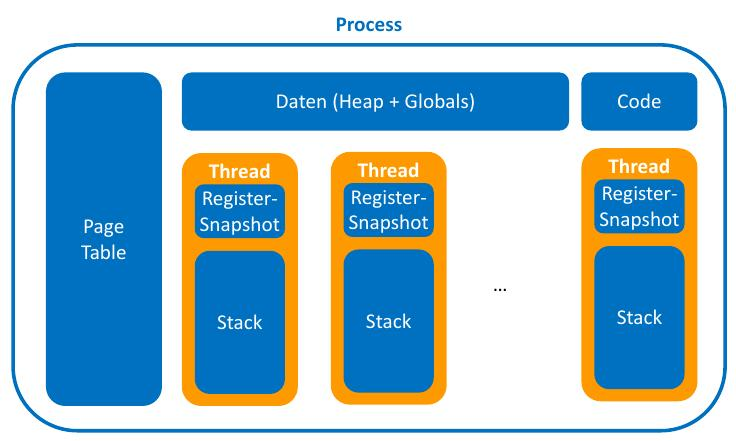
\includegraphics[width=0.7\linewidth]{img/prozess_speicherressourcen}
	\caption{Speicherressourcen eines Prozesses}
	\label{fig:prozessspeicherressourcen}
\end{figure}

\subsection{Threading}
Levels:
\begin{itemize}
	\item User Level: In der Laufzeitumgebung virtualisierte Parallelität
	\item Kernel Level (heute meistens; bei JVM zusätzlich Simulation in der JVM; 1:1 Abbildung)
\end{itemize}


\subsection{Scheduling}
\begin{description}
	\item[Synchron] Vom Programm aus warten. Thread gibt CPU freiwillig frei.
	\item[Asynchron] Prozessor/Scheduling bestimmt Auszeit
\end{description}


\subsubsection{Policies}

\begin{description}
	\item[Kooperativ] Programm macht Unterbruch, Scheduler kann Programm nicht unterbrechen
	\item[Preemtiv] Forcierter Unterbruch (z.B per Timer-Interrupt)
\end{description}

\subsubsection{Java Virtual Machine}
Die JVM ist ein Single Process System. Die JVM erzeugt beim Aufstarten einen Thread, welcher die statische Methode main() aufruft. Der Programmierer kann weitere Threads starten. Auf Deamon Threads (z.B. den Garbage Collector) wird beim Beenden nicht gewartet.

\subsubsection{Java Thread Types}
\paragraph{Einfacher Thread:} \hfill

\begin{lstlisting}[language=java]
class SimpleThread extends Thread { 
	@Override public void run() {
		// parallel execution
	} 
}
Thread myThread = new SimpleThread(); 
mythread.start();
// --> Austritt bei Terminierung run(), oder via Exception, Return oder fertig.
\end{lstlisting}

\paragraph{Thread mit Runnable Interface} \hfill \\
\begin{lstlisting}[language=java]
class SimpleLogic implements Runnable { 
	@Override public void run() {
		// parallel execution
	} 
}
Thread myThread = new Thread(new simpleLogic());
myThread.start();
\end{lstlisting}

\paragraph{Thread mit Lambda} \hfill \\
\begin{lstlisting}[language=java]
Thread myThread = new Thread(() -> {
	// parallel execution
});
myThread.start();
\end{lstlisting}

\subsubsection{Java Thread Commands}
\begin{lstlisting}[language=java]
Thread.sleep(milliseconds) // CPU freigeben und dann wait
Thread.yield(); // CPU freigeben und direkt wieder ready sein.
myThread.join();      // Warten auf return der run();
!myThread.isAlive();  // nach Join ist der Thread nicht mehr am Leben

// In der Praxis oft missbraucht, um Locks zu loesen
myThread.interrupt(); // nur verwendet, wenn Cancel-Policy des Threads bekannt.
Thread.currentThread(); // nie join() auf aktuelle Thread aufrufen
t.setDaemon(boolean on);
\end{lstlisting}

\subsection{Thread Synchronisation}

Oft muss die Nebenläufigkeit der Theads beschränkt werden, damit keine fehlerbehaftete Parallelität besteht. Threads teilen sich:
\begin{itemize}
	\item Instanzvariablen
	\item Statische Variablen
	\item Elemente in einem Array
	\item (Java 8: lokale Variablen nur lesend)
\end{itemize}

Dabei gibt es zwei Fälle:

\begin{description}
	\item[Gegenseitiger Ausschluss] Nur ein Threads kann eine Ressource nutzen (Mutual Exclusion)
	\item[Warten auf Bedingungen] Warten, bis eine Ressource zur Verfügung steht.
\end{description}

Ohne diese Vorkehrungen laufen Threads beliebig verzahnt und verändern im schlimmsten Fall unkontrolliert, gegenseitig die Daten. (Race Conditions)

\subsubsection{Race Condition}

Zwei Threads greifen z.B. parallel auf eine Ressource zu; nach dem auslesen arbeiten beide mit dem alten Wert.
Dies ist ein Fehler aufgrund von unkontrollierter Nebenläufigkeit.

\subsubsection{Java synchronized Methoden}

Funktioniert mit Locking auf Objektebene. (In diesem Beispiel ist der Lock auf dem \lstinline|BankAccount|-Objekt.

\begin{lstlisting}[language=java]
class BankAccount {
	public synchronized void deposit(int amount) {
		this.balance += amount; // critical section
	}
	public synchronized void withdraw(int amount) {
		this.balance -= amount; // critical section
	}
}
\end{lstlisting}

Alternativ kann ein expliziter synchronized Block angelegt werden:

\begin{lstlisting}[language=java]
class Bankaccount {
	public void deposit(int amount) {
		synchronized(this) {
			this.balance += amount; // critical section
		}
	}
}
\end{lstlisting}

Bei \lstinline|static|-Funktionen findet der Lock auf dem Class Object statt (z.B. \lstinline|Test.class|)

\clearpage

\subsection{Thread Monitor}

Funktioniert mit Wait \& Signal Mechanismus. Threads können damit auf Bedingungen warten und signalisieren.


\begin{figure}[h!]
	\centering
	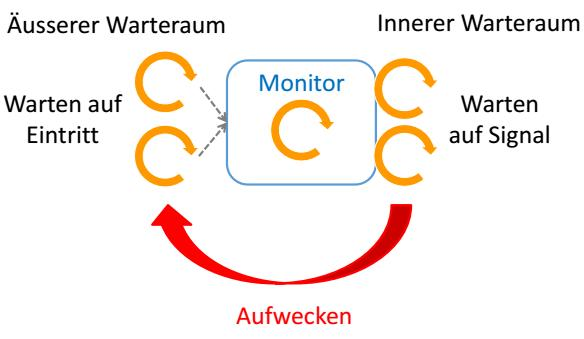
\includegraphics[width=0.7\linewidth]{img/thread_monitor}
	\caption{Thread Monitor}
	\label{fig:threadmonitor}
\end{figure}

\begin{lstlisting}[language=java]
wait(); // warten bis ein Notify eintrifft
notify(); // beliebigen Tread aufwecken (bei .NET FIFO)
notifyAll(); // alle Threads aufwecken (muessen aber synchronized-lock neu akquirieren
\end{lstlisting}


\begin{itemize}
	\item Diese Funktionen funktionieren nur in einem \lstinline|synchronized|-Kontext!
	\item Im Prinzip ist in Java ist ein Spurious Wakeup möglich (d.h. ein aufwachen aus unerfindlichen Gründen)
	\item Ein Aufgeweckter Thread wird nicht immer zwingend direkt in den Monitor genommen.
\end{itemize}

\subsubsection{Object und Class Lock}

\begin{itemize}
	\item Bei mehreren synchronized Methoden kann der Lock genau einmal bezogen werden
	\item Der Lock wird am Ende des Blocks, beim Return Statement oder bei unbehandelten Exceptions wieder freigegeben.
\end{itemize}


\begin{lstlisting}[language=java]
public synchronized void f() { ... } // object lock
public static synchronized void sf() { ... } // class lock (static)

public void f() {
	synchronized(this) { ... } // object lock
}

public static void sf() {
	synchronized(Test.class) { ... } // class lock (static)
}
\end{lstlisting}

\subsubsection{Signal and Continue}
Der signalisierende Thread behält den Monitor auch noch, wenn er \lstinline|notify()| oder \lstinline|notifyAll()| ausgeführt hat. Der aufgeweckte Thread kommt einzig in den äusseren Warteraum und muss dort neu um den Monitor Eintritt kämpfen. In Java gibt es keine garantierte Warteschlange und so kann ein Thread kontinuierlich überholt werden. (Worst Case)



\subsubsection{Typische Fehler}

\begin{itemize}
	\item Monitor mit \lstinline|if(x) wait();| $\rightarrow$ muss immer Schleife sein!
	\item Gegenseitigen Lock von zwei unterschiedlichen Orten kann zu einem gegenseitigen Lock führen $\rightarrow$ Lösung: \lstinline|notifyAll()|, das ist aber ineffizient
\end{itemize}

\subsubsection{Wann reicht eine Single Notify?}

\begin{enumerate}
	\item Nur eine semantische Bedingung (Uniform Waiters): Bedingung interessiert \textbf{jeden} wartenden Thread
	\item Bedingung gilt jeweils nur für einen (One-In/One-Out): Nur ein \textbf{einziger} wartenden Thread
\end{enumerate}

\subsubsection{Vor und Nachteile}
\paragraph{Vorteile}
\begin{itemize}
	\item Jede Synchronisation damit realisierbar
	\item Sychronisation ist in einem OO-Objekt gekapselt
\end{itemize}

\paragraph{Nachteile}
\begin{itemize}
	\item Logik muss eigenständig implementiert werden (\lstinline|synchronized|, \lstinline|wait()|, \lstinline|notify()|, \lstinline|notifyAll()|)
	\item Effizienzprobleme (notifyAll() bei mehreren Conditions)
	\item Fairnessprobleme (Signal and Continue, kein FIFO)
\end{itemize}



\section{Synchronisationsprimitiven}

\subsection{Semaphoren}

Ein Semaphor vergibt eine beschränkte Anzahl an freien Ressourcen an die Threads. Er weiss, wie viele noch frei sind (z.B. freie Parkplätze). 

\begin{description}
	\item[aquire()] Bezieht eine Ressource, wartet, falls keine mehr frei ist. Ansonsten Zähler dekrementieren. Der Methode kann auch ein Integer Wert übergeben werden, um auf einmal mehrere Ressourcen anzufordern.
	\item[release()] Ressource freigeben, Zähler inkrementieren. Der Methode kann auch ein Integer Wert übergeben werden, um auf einmal mehrere Ressourcen freizugeben.
\end{description}

\paragraph{Typen} \hfill \\
Es gibt Binäre (0,1) oder grössere Semaphoren (N). In Java gibt es auch einen negativen Semaphore (nicht so in Windows oder .NET). Binäre Semaphore werden für Mutual Exclusion verwendet.

\paragraph{Fairness} \hfill \\
Faires FIFO ist möglich, wenn als zweiter Konstruktorparameter \lstinline|true| mitgegeben wird: \lstinline[language=java]|new Semaphore(N, true);|. Standardmässig ist auch der Semaphore unfair.

\begin{lstlisting}
class BoundedBuffer<T> {
	private Queue<T> queue = new LinkedList<>();
	private Semaphore upperLimit = new Semaphore(Capacity, true);
	private Semaphore lowerLimit = new Semaphore(0, true);
	private Semaphore mutex = new Semaphore(1, true);
	public void put(T item) throws InterruptedException {
		upperLimit.acquire();
		mutex.acquire(); queue.add(item); mutex.release();
		lowerLimit.release();
	}
	public T get() throws InterruptedException {
		lowerLimit.acquire();
		mutex.acquire(); T item = queue.remove(); mutex.release();
		upperLimit.release();
		return item;
	}
}
\end{lstlisting}

\clearpage

\subsection{Lock \& Conditions}
Lock \& Conditions ist ein spezieller Typ von Monitor. Er ist jedoch vollkommen unabhängig vom Java Monitor. Er verfügt über mehrere Wartequeues für verschiedene Conditions. (kommt aus POSIX, in Windows nicht vorhanden). Er besteht aus zwei Komponenten:

\begin{enumerate}
	\item Lock Objekt: Sperre für den Eintritt in den Monitor
	\item (mehreren) Conditionen Objekte: Wait \& Signal pro Bedingung
\end{enumerate}

\begin{lstlisting}
class BoundedBuffer<T> {
	private Queue<T> queue = new LinkedList<>();
	private Lock monitor = new ReentrantLock(true);
	private Condition nonFull = monitor.newCondition();
	private Condition nonEmpty = monitor.newCondition();
	
	public void put(T item) throws InterruptedException {
		monitor.lock(); 
		try {
			while (queue.size() == Capacity) { nonFull.await(); }
			queue.add(item);
			nonEmpty.signal();
		} finally { monitor.unlock(); }
	}
	public T get() throws InterruptedException {
		monitor.lock(); 
		try {
			while (queue.size() == 0) { nonEmpty.await(); }
			T item = queue.remove();
			nonFull.signal();
			return item;
		} finally { monitor.unlock(); } 
	}
}
\end{lstlisting}

\subsection{Read-Write Lock}
Bei rein lesenden Zugriffen kann auf gegenseitigen Ausschluss verzichtet werden. Gibt es aber nur einen schreibenden Teilnehmer, braucht es dringen gegenseitigen Ausschluss.

\begin{lstlisting}[language=java]
ReadWriteLock rwLock = new ReentrantReadWriteLock(true); 

rwLock.readLock().lock(); //true->fair
// paralell  read only access
rwLock.readLock().unlock();

rwLock.writeLock().lock();
// exclusive write (and read) access
rwLock.writeLock().unlock();
\end{lstlisting}


\subsubsection{RWLock mit Conditions}

Es ist möglich, eine Condition auf ein Write-Lock zu setzten.

\begin{figure}[h!]
	\centering
	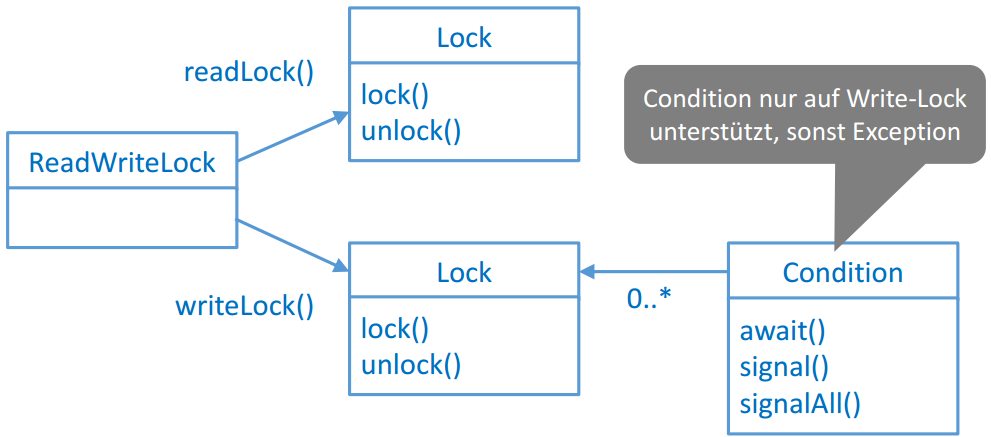
\includegraphics[width=0.7\linewidth]{img/rw_lock_conditions}
	\caption{Read-Write Lock mit Conditions}
	\label{fig:rwlockconditions}
\end{figure}

\clearpage

\subsection{Synchronisationspunkt}
Mehrere Threads warten auf eine Bedingunge. Sobald die Bedingung erfüllt ist, laufen alle weiter.

\subsubsection{Count Down Latch}
Der Count Down Latch zählt so lange herunter, bis der Zähler kleiner, gleich 0 wird. Ein Latch kann im Gegensatz zu einer Lösung mit Semaphoren genau einmal verwendet werden.

\begin{lstlisting}
CountDownLatch carsReady = new CountDownLatch(N); // wait for N cars
CountDownLatch startSignal = new CountDownLatch(1); // give signal

// N Cars count down
carsReady.countDown();
startSignal.await();

// Race control waits and gives signal
carsReady.await();
startSignal.countDown();
\end{lstlisting}

\subsubsection{Cyclic Barrier}

Treffpunkt für fixe Anzahl Threads. Threads warten (mit \lstinline|await()|), bis alle angekommen sind. Ist im Gegensatz zum CountDownLatch wiederverwendbar. Die Anzahl Teilnehmer werden beim Konstruktor gesetzt und können nicht mehr geändert werden.

\begin{lstlisting}
CyclicBarrier raceStart = new CyclicBarrier(N); // Race control
raceStart.await(); // N cars

// repeatable cyclinc barrier
CyclicBarrier gameRound = new CyclicBarrier(N);
while(true) {
	gameRound.await();
}
\end{lstlisting}


\subsubsection{Phaser}
Veralgemeinerte Cyclic Barrier implementation in Java. Der Phaser wird eher selten bis nie verwendet.


\subsubsection{Rendez-Vous: Exchanger}
Warten auf einen zweiten Prozess und austauschen von Daten an diesem Punkt. Es gibt genau zwei Parteien.

\begin{lstlisting}[language=java]
Exchanger<V> e = new Exchanger<>();

e.exchange(objA);
e.exchange(objB);
\end{lstlisting}


\section{Gefahren der Nebenläufigkeit}

Nebenläufige Fehler sind oft schwierig zu erkennen, da sie nicht deterministisch auftreten.

\subsection{Race Conditions}

% TODO was ist hier genau gemeint?
Ungenügend synchronisierte Zugriffe auf gemeinsame Ressourcen. Ursache ist oft ein Data Race, der unsynchronisierter Zugriff auf die gleiche Variable/Speichern. Dabei kann es zu Lost Updates kommen, da aufgrund von Optimierungen enge Read/Write Aktionen getrennt werden können.

\begin{lstlisting}[language=java]
account.setBalance(account.getBalance() + 100);
\end{lstlisting}

Eine Race-Condition kann aber auch aufgrund eines Unterbruchs zwischen Read und Write entstehen (kein atomarer Zugriff).

Critical Sections zur Vermeidung von Race Conditions können nicht statisch erkannt werden, sondern nur vom Entwickler.

\subsubsection{Data Race}
Ein Data Race ist, wenn zwei Instruktionen von unterschiedlichen Threads die gleiche Memory Location bearbeiten und mindestens einer davon eine Write Zugriff ist. Gibt es keine Synchronisation zwischen den beiden Threads gibt es einen Data Race. Dahingegen ist eine Race Condition mehr ein sematischer Fehler, der wegen ungünstiger Reihenfolge oder Timing der Events zu einem fehlerhaften Verhalten der Software führt.

\paragraph{Bedingugen für einen Data Race}
\begin{itemize}
	\item Nebenläufigkeit
	\item auf die gleiche Variable
	\item Nicht synchronisiert
	\item Mindestens ein Schreibzugriff
\end{itemize}

\subsubsection{Lösungen}
Synchronisation ist relativ teuer, es lohnt sich deshalb nicht, einfach alles zu synchronisieren. Race Conditions sind sogar mit Synchronisation möglich.
\begin{itemize}
	\item Immutability (Unveränderlichkeit)
		\begin{itemize}
			\item Objekte mit nur lesendem Zugriff (\lstinline|final|)
		\end{itemize}
	\item Confinement (Einsperrung)
		\begin{itemize}
			\item Objekt gehört nur einem Thread zu einer Zeit (Thread Confinement)
			\item Meistens Klasse, welche den Zugriff und die Daten kapselt (Object Confinement)
			\item Eine Falle: Bei z.B. Übergabe einer Liste gibt es immer noch Referenzen nach aussen.
		\end{itemize}
\end{itemize}

\paragraph{Thread Confinement} \hfill
\begin{lstlisting}
void service() {
	new Thread(() -> {
		// object only accessible within thread
		OutputStream output = new FileOutputStream("..");
		try {
			doService(output);
		} finally {
			output.close();
		}
	}.start();
}
void doService(OutputStream s) {
	// s must not be passed to other threads
}
\end{lstlisting}

\paragraph{Object Confinement} \hfill \\
Bei Object Confinement muss man darauf achten, dass die Kapselung durch z.B Rückgabe von Objektreferenzen nicht gebrochen werden!
\begin{lstlisting}
class ProductDatabase {
	// enclosed variable (private)
	private HashMap<String, Product> productMap = new HashMap<>();
	public synchronized void addProduct(String name, String details) {
		productMap.put(name, new Product(details));
	}
	public synchronized String getProductDetails(String name) {
		return productMap.get(name).getDetails();
	}
	public synchronized void notifySale(String name) {
		productMap.get(name).increaseSales();
	}
}
\end{lstlisting}


\subsubsection{Thread Safety}

Es gibt keine einheitliche Definition für ''Thread Safety''. Üblicherweise ist damit gemeint, dass:
\begin{itemize}
    \item keine Race Conditions im Code existieren
    \item kritische Abschnitte nur pro Methode erfüllt werden.
\end{itemize}

Es kann also immer noch zu anderen Fehlern kommen. Darum: Immer Spezifikation prüfen!

\subsubsection{Java Collections und Thread Safety}

Vector, Stack, Hashtable (Java 1.0 Collections) und alle Concurrent Collections sind Thread Safe, die normalen Datenstrukturen (HashSet, TreeSet, ArrayList, LinkedList, HashMap, TreeMap) nicht. Man verzichtet dabei bewusst auf den Overhead, da Thread-Sicherheit im Normalfall nicht benötigt wird.


\paragraph{Verstecktes Multi Threading in Java}
Finalizers, Timers und evtl. externe Libraries können in eigenen Threads laufen, ohne das dies explizit angegeben wurde.

\subsection{Deadlocks}

Gegenseitige Aussperrung von Threads, so dass keiner von ihnen weitermachen kann.

\paragraph{Nested Locks} \hfill
\begin{lstlisting}
// thread 1
synchronized(listA) { 
	synchronized(listB) {
		listB.addAll(listA);
	}
}

// thread 2
synchronized(listB) { 
	synchronized(listA) {
		listA.addAll(listB);
	}
}
\end{lstlisting}

\paragraph{Livelocks} \hfill \\
Livelocks sind Deadlocks, welche aber vorzu noch aktiv CPU-Zeit verbrauchen
\begin{lstlisting}
// thread 1
b = false;
while (!a) { sleep(1); }

// thread 2
a = false;
while (!b) { sleep(1); }
\end{lstlisting}



\paragraph{Deadlock Erkennung} \hfill \\
Deadlocks können mit einem Betriebsmittelgraph erkannt werden. Gibt es einen Zyklus im Graphen, hat man es mit einem Deadlock zu tun. Damit es zu einem Deadlock kommt, müssen folgende vier Bedingungen zutreffen:
\begin{itemize}
	\item Geschachtelte Locks
	\item Zyklische Warteabhängigkeiten
	\item Gegenseitiger Ausschluss (Locks)
	\item Sperren ohne Timeout/Abbruch
\end{itemize}

\paragraph{Deadlock Vermeidung} \hfill \\
Deadlocks können mit folgenden Techniken vermieden werden:
\begin{itemize}
	\item Lineare Ordnung der Ressourcen einführen (z.B In aufsteigender Reihenfolge locken)
	\item Grobgranulare Locks: Sperre das Parent Objekt (z.B Bank bei Kontozugriff sperren)
\end{itemize}

\subsection{Starvation}
Kontinuierliche Fortschrittsbehinderung von Threads aufgrund von Fairness-Probleme. Ein Thread bekommt also nie die Chance, auf eine Ressource zuzugreifen. Thread Prioritäten können zu Starvation führen. Starvation kann vermieden werden, wenn man faire Synchronisationskonstrukte verwendet. 


\section{Thread-Pool}

Tasks sind Beschreibungen von Aufgaben, welche parallel ausgeführt werden dürfen, es aber nicht müssen.

Tasks in der Task Queue werden von einer beschränkten Anzahl von Worker Threads im Thread Pool abgearbeitet.

\paragraph{Vorteile}
\begin{itemize}
	\item Beschränkte Anzahl von Threads: Erhöht Effizienz, da weniger Overhead
	\item Recycling der Threads: Spart Overhead eines Threads
	\item Höhere Abstraktion: Der ''Problem Space'' wird vom ''Machine Space'' getrennt.'
	\item Anzahl vernünftiger Threads pro System konfigurierbar: \#Worker Threads = \#Prozessoren + \#I/O-Aufrufe. Oft werden so viele Threads bereitgestellt, wie es logische Prozessoren gibt.
\end{itemize}

\paragraph{Nachteile}
\begin{itemize}
	\item Programme müssen neu als Tasks mit den entsprechenden Einschränkungen modelliert werden
	\item Deadlocks bei gegenseitigen Abhängigkeiten möglich
	\item Task muss zu Ende laufen, bevor ein anderer Ausgeführt werden kann, da der Stack nicht einfach persistiert werden kann.
	\item Ausnahme: Geschachtelte Tasks (Sub-Tasks)
\end{itemize}

\subsubsection{Fork-Join-Pools}
Seit Java 7 gibt es Fork-Join-Pools, welche eine effiziente und rekursive Aufgaben unterstützten

\begin{lstlisting}[language=java]
ForkJoinPool threadPool = new ForkJoinPool();
Future<Integer> future = threadPool.submit(() -> {
	int value = ...; // long calculation
	return value; // optional return value
});
\end{lstlisting}

\subsubsection{Future Konzept}

Future-Promises sind Werte, die zum aktuellen Zeitpunkt noch nicht feststehen, aber demnächst zurückgeliefert werden sollen.

\begin{lstlisting}[language=java]
Future<T> future = threadPool.submit(...);
//...
T result = future.get(); // Blockierend auf Wert warten.
\end{lstlisting}

\paragraph{Exceptions}, welche während der Ausführung entstehen, werden in eine \lstinline|ExecutionException| geschachtelt und dann beim \lstinline|get()| zurückgegeben.

\paragraph{Ein Task Abbruch} kann mit \lstinline[language=java]|cancel(boolean mayInterruptIfRunning)| durchgeführt werden. Cancel ist standardmässig Kooperativ und nimmt alle Tasks aus der Queue heraus, kann optional aber auch Interrupts an laufende Prozesse senden senden.

\paragraph{Tasks ohne Returns} sind möglich, aber Achtung, Exceptions darin werden nicht behandelt, ausser es wird ein \lstinline|get()| ausgeführt. Diese werden in Daemon-Threads ausgeführt, bei Programmende werden diese also beendet! (Fire and Forget)

\paragraph{Über-Parallelisierung} Ab einem bestimmten Schwellwert von Teilproblemen ist die parallele Variante langsamer wie eine sequenzielle Bearbeitung des Problems. Dies rührt daher, dass die Parallelität auch immer einen bestimmten Overhead mit sich bringt. Gerade bei rekursiven Konstrukten lohnt es sich deshalb, eine minimale Grösse des Teilproblems zu definieren.

\subsubsection{Rekursive Subtasks}

\begin{lstlisting}[language=java]
class CountTask extends RecursiveTask<Integer> {
	private final int lower, upper; 
	
	public CountTask(int lower, int upper) {
		this.lower = lower; this.upper = upper;
	}
	
	@Override
	protected Integer compute() {
		if (upper - lower > THRESHOLD) { 
			// parallel count
			int middle = (lower + upper) / 2;
			CountTask left = new CountTask(lower, middle); 
			CountTask right = new CountTask(middle, upper);
			left.fork(); 
			right.fork();
			return right.join() + left.join();
		} else {
			// sequential count
			int count = 0;
			for (int number = lower; number < upper; number++) {
				if (isPrime(number)) { 
					count++; 
				}
			}
			return count;
		}

	}
}

ForkJoinPool threadPool = new ForkJoinPool();
Future<Integer> result = threadPool.invoke(new CountTask(2, INPUT_SIZE));
\end{lstlisting}

\begin{figure}[h]
	\centering
	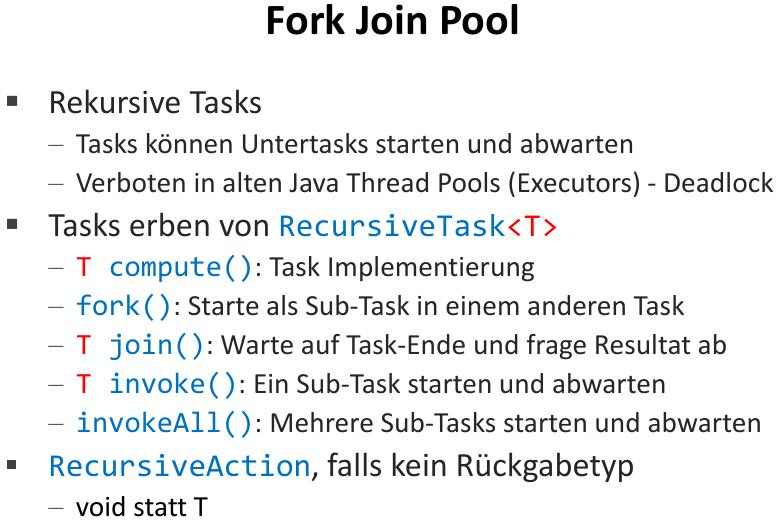
\includegraphics[width=0.7\linewidth]{img/fork_join_pool}
	\caption{Fork Join Pool API}
	\label{fig:forkjoinpool}
\end{figure}

\subsubsection{Work Stealing Verfahren}

Globale Queue (FIFO), sowie Verteilung eine lokale Queues (LIFO) pro Thread. Bei einer Überlastung eines Threads werden Tasks umverteilt, was als Work Stealing bezeichnet wird.

\paragraph{Vorteil}: Es muss nicht immer ein globaler Lock akquiriert werden.


\subsection{Asynchrone Programmierung: CompletableFutures}

In der klassischen prozeduralen Programmierung gibt es viele blockierende Aufrufe: Das ist ineffizient. 

Ab Java 8 ist daher dies möglich: 
\begin{lstlisting}[language=java]
CompletableFuture<Long> future = CompletableFuture.supplyAsync(() -> longOperation());
// Einsatz von runAsync, falls es keinen Rueckgabewert gibt.
//other work
process(future.get());
\end{lstlisting}

\paragraph{Caller-zentrisch} Der Caller wartet auf das Ende des Tasks und holt sich das Resultat vom Future (Pull)

\paragraph{Callee-zentrisch} Der Callee informiert den Caller über das Resultat. Man erreicht dies mit Continuation und Promises. (Push)

\subsubsection{Continuation / Promise}
Sobald der erste Task abgeschlossen ist, wird die Folgeaufgabe ausgeführt. Diese kann in einem beliebigen Worker-Thread ausgeführt werden.

Bei Continuation / Promises müssen die Probleme der Asynchronen Programmierung beachtet werden.

\begin{itemize}
	\item \lstinline|thenAccept()| für Handler ohne Rückgabe
	\item \lstinline|thenApply()| für Funktionen mit Rückgabe
\end{itemize}

\begin{lstlisting}[language=java]
// Multi continuation
CompletableFuture.allOf(future1, future2).thenAccept(continuation);
CompletableFuture.any(future1, future2).thenAccept(continuation);

// Single continuation
CompletableFuture<Long> future = CompletableFuture.supplyAsync(() -> longOperation());
// ...
future.thenAccept(result -> System.out.println(result)).thenApply(future3); // muss nicht asynchron sein.
future.thenAcceptAsync(result -> System.out.println(result)).thenApplyAsync(future3); // asynchrone anwendung -> garantiert asynchron
\end{lstlisting}


\subsection{Java 8 Stream API}

\begin{figure}[h]
	\centering
	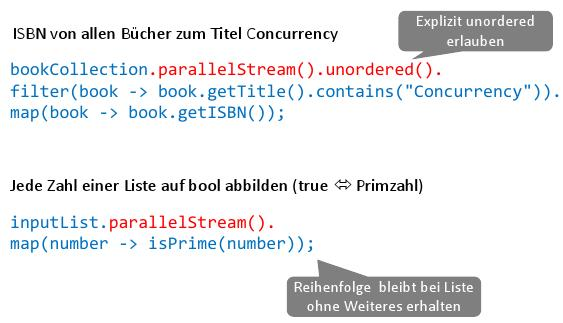
\includegraphics[width=0.7\linewidth]{img/java8_stream_api}
	\caption{Java 8 Stream API}
	\label{fig:java8streamapi}
\end{figure}


\section{.NET / C\#}
\lstset{style=visual-studio-style}
Die C\# Laufzeit Umgebung beinhaltet die .NET Task Parallel Library (TPL), welche viele nütztliche Funtionen zur Verfügung stellt. 

\begin{itemize}
	\item Es gibt zusätzlich ReadWritLockSlim für Upgradeable Read/Write
	\item Semaphore und Mutex (binärer Semaphore) sind auch auf OS Stufe nutzbar
	\item Es gibt kein Fairness Flag
	\item Es gibt kein Lock \& Condition
	\item Wie in Java sind die Collection nicht Thread-safe (Ausser System.Collections.Concurrent)
\end{itemize}

\subsection{Monitor}
\begin{itemize}
	\item Der Monitor unter C\# informiert immer den am längsten wartenden Thread (in Java ist dies nicht deterministisch).
	\item Ebenfalls gibt es unter .NET kein Spurious Wakeup (aufwachen aus untergründlichen Gründen).
	\item Wie in Java muss in einer \lstinline|while| Schleife gewartet werden, da ansonsten Probleme mit Signal and Continue auftreten. 
	\item Locks auf das \lstinline|this| Objekt sind in der C\# Gemeinde nicht gerne gesehen. Um diese nicht zu verägern, sollte man deshalb ein generelles \lstinline|object| ohne Funktionalität erstellen. 
\end{itemize}

\begin{figure}[h]
	\centering
	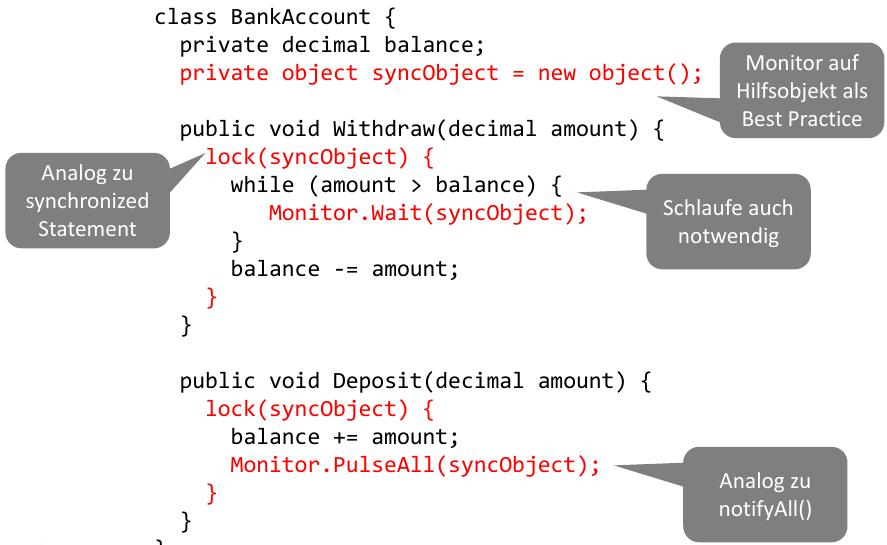
\includegraphics[width=0.7\linewidth]{img/csharp_monitor}
	\caption{CSharp Monitor}
	\label{fig:csharpmonitor}
\end{figure}

\subsection{Threads}
Threads sind in C\# konservativer implementiert. Git es eine Exception in einem Thread, wird das Programm abgebrochen. (in Java läuft es weiter). Ebenfalls wird oft nicht von Thread geerbt, sondern direkt ein Lamda übergeben. Im Gegensatz zu Java kann ein Lamda in C\# auf die umgebenden Variablen zugreifen. (In Java sind diese implizit \lstinline|final|). Beim schreibenden Zugriff auf umliegende Variablen ist aber Vorsicht geboten. Die Zugriffe sind prädestiniert für Data Races!


\begin{lstlisting}[language={[Sharp]C}]
	bool aVariable = false;
	Thread myThread = new Thread(() => {
		aVariable = true; // Achtung, gefaehrlich fuer Data Races.
	});
	
	myThread.Start();
	// ... Bei exceptions: Effekt auf ganze Applikation -> es gibt einen Globalen Fehler.
	myThread.Join();
\end{lstlisting}

\subsection{Work Stealing Thread Pool}
Der Work Stealing Thread Pool wurde in -NET 4 eingeführt und gehört zu den modernsten Thread Pools. Es beinhaltet:
\begin{itemize}
	\item Task Paralellization: Explizite Tasks starten und warten
	\item Data Parelellization: Paraellele Statements und Queries
	\item Asynchronous Programming: Mit Continuation Style.
\end{itemize}

\subsection{Tasks}
\begin{itemize}
	\item Tasks können auf Subtasks warten, ohne dass ein spezieller ForkJoinTask nötig wäre
\end{itemize}

\begin{lstlisting}[language={[Sharp]C}]
Task task = Task.Run(() => {
	// task implementation
});

// perform other activity
task.Wait();
\end{lstlisting}

und mit Rückgabe:
\begin{lstlisting}[language={[Sharp]C}]
Task<int> task = Task.Run(() => { 
	int total = ...;
	// some calculation return total;
});

//...
Console.Write(task.Result); // task.Result ist ein Blockierendes Wait!
\end{lstlisting}

\subsection{Thread Injection}
Die TPL fügt zur Laufzeit neue Worker Threads hinzu, wenn welche benötigt werden. Dabei wird Durchsatz gemessen und gemäss diesem die Anzahl an Worker Threads dynamisch vergrössert/verkleinert. (Hill Climbing Algorithmus). Das Problem dabei ist, dass somit nie Deadlocks entstehen können, da immer weitere Worker Threads hinzugefügt werden. (Massnahme: \lstinline|ThreadPool. SetMaxThreads()|)

\subsection{Datenparallelität in TPL}
\begin{lstlisting}[language={[Sharp]C}]
Paralell.Invoke(
	() => MergeSort(l, m),
	() => MergeSort(m, r)
); // Implizites WaitAll

Paralell.ForEach(list,
	file => Convert(file)
); // Implizites WaitAll


Paralell.For(0, array.Length,
	i => DoComputation(array[i])
);
\end{lstlisting}

\subsection{Partitionierung} 

\paragraph{Range Partitioners} (Paralell.For und Invoke) macht zusammenhängende Blöcke, da das Maximum bekannt ist. 

\paragraph{Striped Partitioners} (Paralell.ForEach) wird aufgrund eines Modulos verteilt. (Häufig angewendet, wenn nicht klar ist, wie viele Elemente vorhanden sind. z.B bei Iteratoren)


\subsection{Paralell LINQ (PLINQ)}
LINQ ist eine an SQL angelehnte Abfragesprache auf das Objektmodell. PLINQ ist erlaubt eine paralle Verarbeitung dieser Abfragen. Auch hier muss darauf geachtet werden, dass sicher keine Seiteneffekte (Race Conditions, Deadlocks) existieren!
\begin{figure}[h]
	\centering
	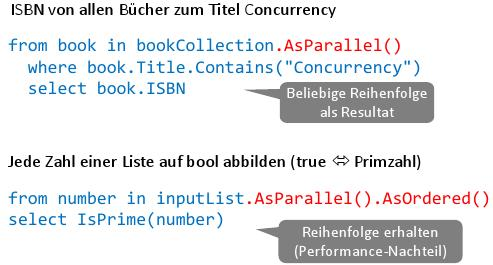
\includegraphics[width=0.6\linewidth]{img/csharp_linq_paralell}
	\caption{Paralell LINQ}
	\label{fig:csharplinqparalell}
\end{figure}


\subsubsection{Paralelle Queries}
Mit PLINQ können Daten parallel geladen und forlaufend verarbeitet werden. Man benötigt dazu die Klasse \lstinline|ParallelQuery|.
\begin{figure}[h]
	\centering
	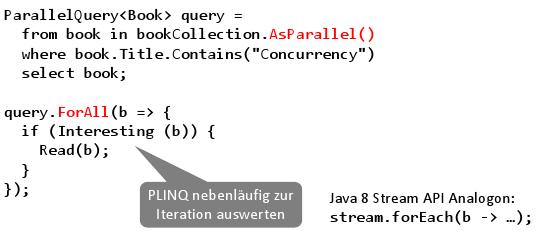
\includegraphics[width=0.7\linewidth]{img/csharp_plinq}
	\caption{PLINQ}
	\label{fig:csharpplinq}
\end{figure}

\subsection{Asynchrone Programmierung}
\begin{lstlisting}[language={[Sharp]C}]
var task = Task.Run(
	// long operation
);

int result = task.Result;
\end{lstlisting}

\subsection{Task Continuations}
\begin{lstlisting}[language={[Sharp]C}]
task1.
	ContinueWith(task2).
	ContinueWith(task3); // ContinueWith uebergibt einen Parameter mit dem Return des Vorgaengers

// Multi-Continuation
Task.WhenAll(task1, task2).ContinueWith(continuation);
Task.WhenAny(task1, task2).ContinueWith(continuation);
\end{lstlisting}


\section{Threading und GUIs}

Das GUI wird durch den einzelnen UI-Thread ausgeführt; dieser ist der einzige, welche auf Komponenten zugreifen kann. Er besteht aus einer Event Loop; der Thread funktioniert wie ein Worker-Thread. Folglich sollte keine aufwändige Arbeiten im GUI Thread ausgeführt werden, da ansonsten das GUI eingefriert. 

\begin{figure}[h!]
	\centering
	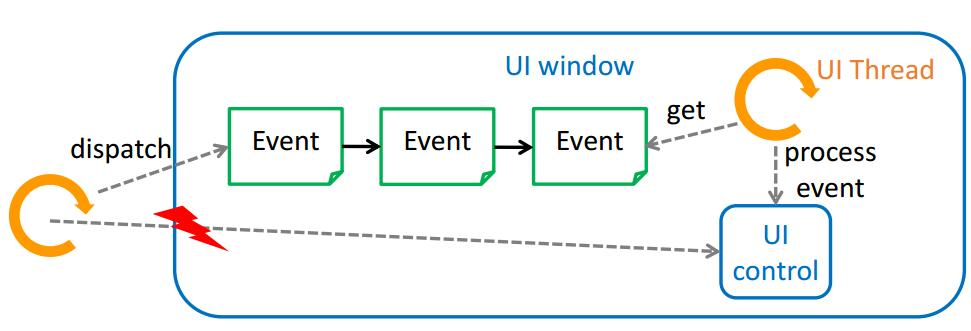
\includegraphics[width=0.7\linewidth]{img/gui_thread_model}
	\caption{GUI Single Thread Model}
	\label{fig:guithreadmodel}
\end{figure}

\subsection{UI Thread Confinement}
Unter Thread Confinement versteht man, dass nur der UI Thread auf UI komponenten zugreifen darf. Andere Threads dürfen nicht direkt auf die UI Komponenten zugreifen und müssen sich als Event inder UI Event Queue einreihen.

\subsection{Java UI Thread}

UI-Thread wird auch als Event Dispatching Thread (EDT) bezeichnet.

\subsubsection{GUI Implikationen}

\begin{description}
	\item[Keine langen Operationen in UI Thread] sonst blockiert das UI
	\item[Kein Zugriff aus anderen Threads] sonst kann es zu Race-Conditions kommen.
\end{description}



\subsubsection{Swing Dispatcher} 
Für das Dispatching wird unter Swing die Klasse \lstinline|SwingUtilities| verwendet. 

\begin{lstlisting}
// async (empfohlen)
static void invokeLater(Runnable doRun);

// sync
static void invokeAndWait(Runnable doRun);

// dispatching example
button.addActionListener(event -> {
	CompletableFuture.runAsync(() -> {
		String text = readHugeFile();
		SwingUtilities.invokeLater(() -> {
			textArea.setText(text);
		});
	});
});
\end{lstlisting}

GUI Aufsetzten geht folgendermassen:

\begin{lstlisting}[language=java]
// frame = ...
SwingUtilities.invokeLater(() -> {
	frame.pack();
	frame.setVisible(true);
});
\end{lstlisting}

\subsubsection{Swing Background Worker}
Bei Swing gibt es auch Swing-Background Worker zur Auslagerung von aufwändigen Operationen:
\begin{figure}[h]
	\centering
	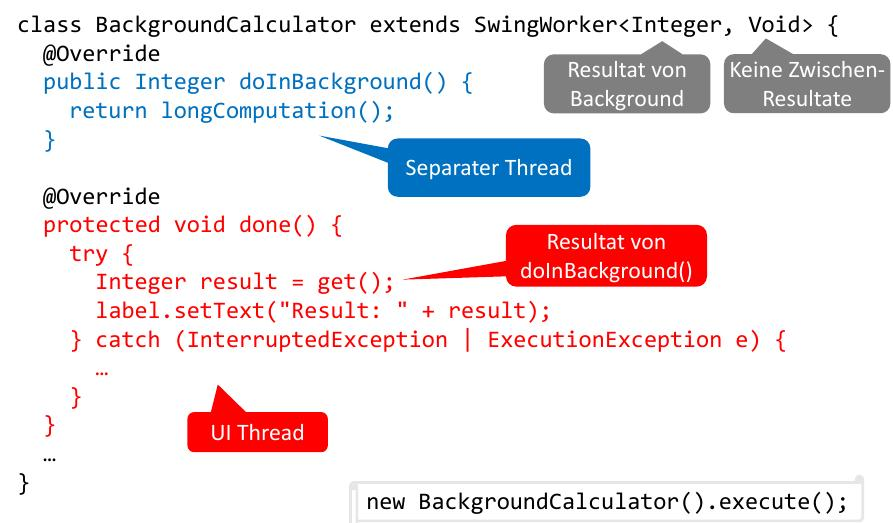
\includegraphics[width=0.7\linewidth]{img/java_swing_background_task}
	\caption{Swing Background Task}
	\label{fig:javaswingbackgroundtask}
\end{figure}


\subsection{.NET UI Threading Modell}
Auch in .NET gibt ein Single Thread Apartment (Confinement). Hier gibt es jedoch keinen bestimmten UI Thread, sondern ein jeder Thread kann der UI Thread werden.

\subsubsection{WPF}
Bei WPF ist der Main Thread implizit auch der GUI-Thread.

\begin{lstlisting}
// WPF: control.Dispatcher.BeginInvoke(delegate)
Task.Factory.StartNew(() => {
	int result = LongCalculation(number);
	Dispatcher.BeginInvoke(new ThreadStart(() => {
		resultLabel.Content = result;
	}));
});
\end{lstlisting}

\subsection{Async/Await}
Das klassische Modell mit den Dispatcher führt zu relativ unleserlichem Code. Deshalb gibt es in .NET ein Compiler Konstrukt, welches diese Logik vor dem Programmierer versteckt. Man benötigt dazu die beiden Keywörter \lstinline|async| und \lstinline|await|. Async Methoden können \lstinline|void|, \lstinline|Task| (Keine Rückgabe, erlaubt trotzdem Warten auf das Ende), \lstinline|Task<T>| zurückgeben und dürfen keine \lstinline|ref| oder \lstinline|out| Parameter enthalten. Async Methoden sind nicht per se asynchron (falls kein await vorhanden)

\begin{lstlisting}[language={[Sharp]C}]
public async Task<int> LongOperationAsync { ... }

// Moegliche Typen: void, Task, Task<T>. Keine "ref" und "out" Parameter.
Task<int> task = LongOperationAsync();
// OtherWork();
int result = await task;

\end{lstlisting}

\begin{figure}[h]
	\centering
	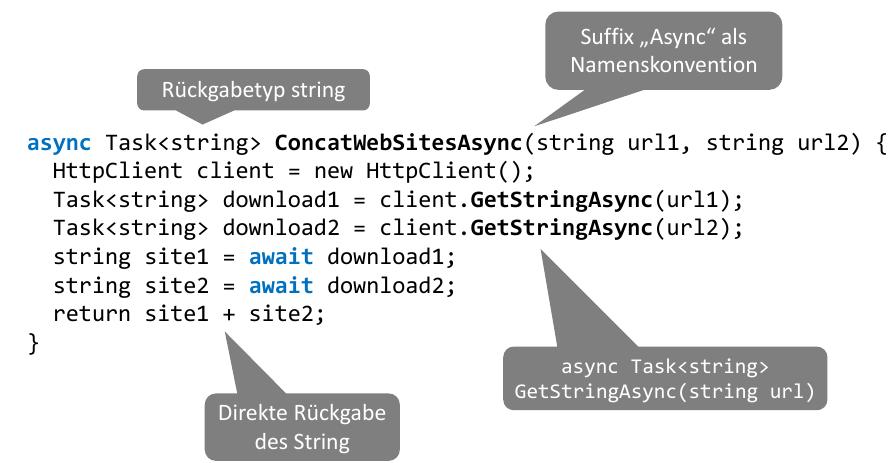
\includegraphics[width=0.7\linewidth]{img/csharp_async_method}
	\caption{CSharp Async Method}
	\label{fig:csharpasyncmethod}
\end{figure}

Eine Async-Methode wird eigentlich in zwei Threads ausgeführt:
\begin{figure}[h]
	\centering
	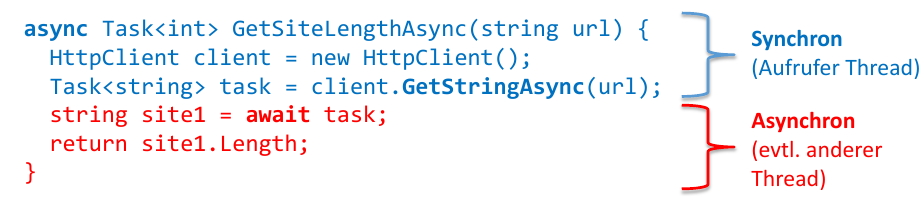
\includegraphics[width=0.7\linewidth]{img/csharp_async_threads}
	\caption{CSharp Async Exceution Threads}
	\label{fig:csharpasyncthreads}
\end{figure}

\subsubsection{Ablauf}
Der Compiler zerlegt jede \lstinline|async| Methode in zwei Abschnitte
\begin{enumerate}
	\item Erster Abschnitt vor Await, welcher synchron ausgeführt wird. Ist man beim \lstinline|await| angekommen, sprint man zurück zum Aufrufer.
	\item Zweiter Abschnitt nach Await, welcher nach dem Task Ende ausgeführt wird.
\end{enumerate}

Man unterscheidet zwischen zwei Fällen von Aufrufer:

\paragraph{Fall 1: Kein UI Thrad}
Der Teil vor dem \lstinline|await| wird im Aufrufer Thread ausgeführt. Der Teil nach dem \lstinline|await| wird im neu gestarteten TPL Thread des aufwändigen Funktion ausgeführt.

\paragraph{Fall 2: UI Thread}
In diesem Fall wird nach Abschluss der aufwändigen Funktion wieder der UI Thread benachrichtig und alle Aktionen werden somit im UI Thread ausgeführt. (Big Benefit)
\begin{figure}[h!]
	\centering
	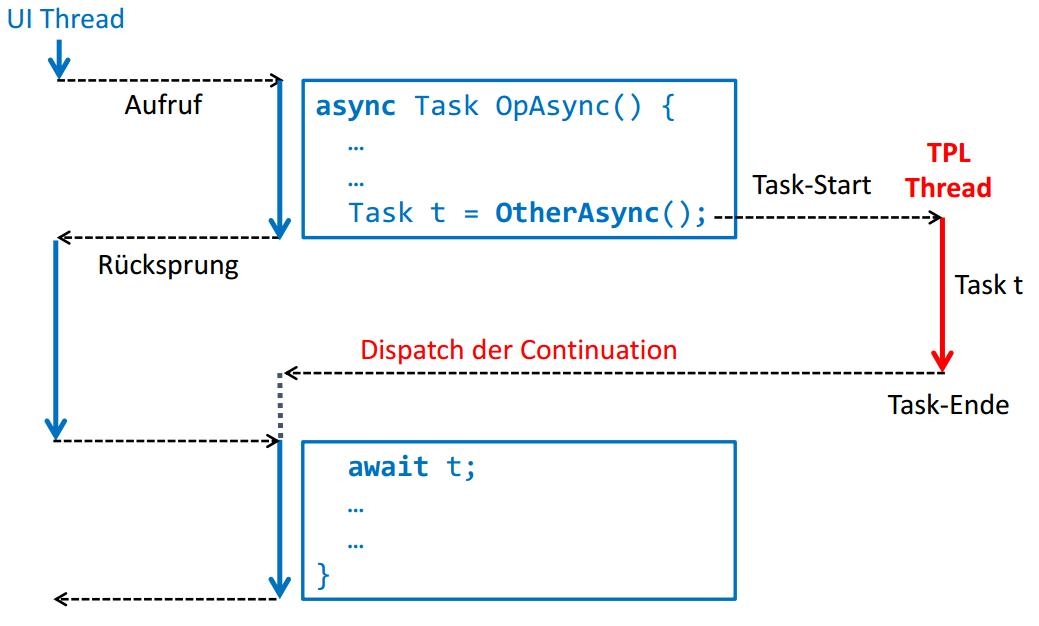
\includegraphics[width=0.7\linewidth]{img/async_await}
	\caption{Async/Await}
	\label{fig:asyncawait}
\end{figure}

Async Methoden sind darum vor allem in UI-Threads sinnvoll. Es gibt dabei ein paar unschöne Design-Entscheidungen, weshalb damit vorsichtig umgegangen werden.


\lstset{style=eclipse-style}

\section{Memory Models}
Für eine effiziente Synchronisation, kann auf Garantien des Speichermodell zurückgegriffen werden. Das Problem ist, dass Compiler, Laufzeitsysteme und CPU's die Instruktionen allenfalls umordnet/wegoptimieren. Sofern der Code nicht synchronisiert ist, treten deswegen Inkonsistenzen auf. (Weak Consitency)

\subsection{Java Memory Model}
In Java gibt es minimale Garantien im Memory Model

\subsubsection{Atomacity}
Atomacity bedeutet, dass der Zugriff auf eine Variable unteilbar duchgeführt wird. Es bedeutet jedoch nicht, dass der Wert einer Variable auch für einen anderen Thread sichtbar ist. Primitive Datentypen (32Bit) und Objekt Referenzen (32 und 64 Bit) sind in Java lesend und schreibend atomar. Bei 64Bit Datentypen (long und double) muss dafür das Keyword \lstinline|volatile| verwendet werden. 

\paragraph{Beispiele} \hfill
\begin{lstlisting}
// Atomar?
int i = 1; 					// nein, da default init (r/w)
long l = -1; 				// nein, da long
l = 42;						// nein, da long
++i; 						// nein, da r/w
String s = "first";		 // nein, da default init (r/w)
s = "second"; 				// atomar, da nur Write der Referenz (String Pooling)
s = null; 					// atomar, nur schreiben
%\end{lstlisting}

\subsubsection{Visibility}
Sichtbarkeit ist bei folgenden Dingen garantiert:
\begin{itemize}
	\item Locks Release \& Acquire: Änderungen vor Release werden bei Acquire sichtbar
	\item Volatile Variablen: Zugriff macht Änderungen anderen Zugreifer sichtbar
	\item Initialisierung von final Variablen: Nach Ende des Konstruktors
	\item Thread-Start and Join: Ebenso Task Start und Ende
\end{itemize}

\paragraph{Beispiele} \hfill
\begin{figure}[h!]
	\centering
	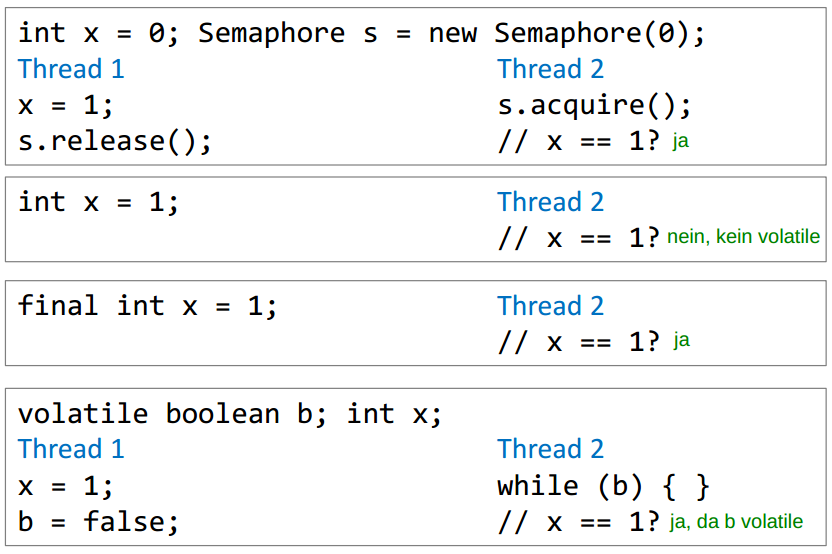
\includegraphics[width=0.6\linewidth]{img/memory_model_visibility}
	\caption{Memory Model Visiblity}
	\label{fig:memorymodelvisibility}
\end{figure}

\newpage

\subsubsection{Ordering}
Es dürfen nur Dinge umgeordnet werden, die nichts miteinander zu tun haben. (Innerhalb eines Threads: «As-If-Serial» Semantik). Zwischen mehreren Threads bleibt Reihenfolge nur erhalten für
\begin{itemize}
	\item Synchronisationsbefehle
	\item Zugriffe auf volatile Variablen
\end{itemize}
Es gibt Keine Umordnung über Synchronisation oder 
volatile Zugriffe hinweg
(Memory Barriers / Memory Fences)

\paragraph{Beispiele} \hfill
\begin{figure}[h!]
	\centering
	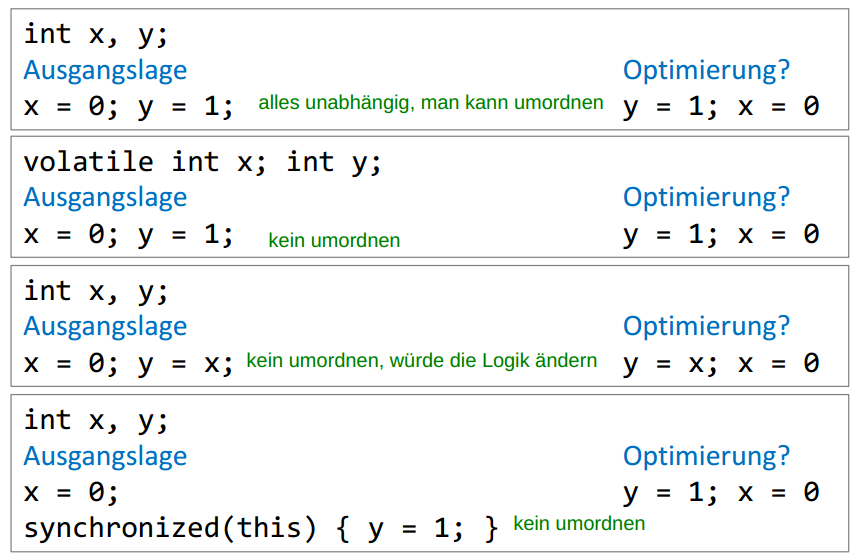
\includegraphics[width=0.6\linewidth]{img/memory_model_ordering}
	\caption{Memory Model Ordering}
	\label{fig:memorymodelordering}
\end{figure}


\subsection{Volatile}
Das \lstinline|volatile| Keyword verhindert Data Races auf Variablen:
\begin{description}
	\item[Atomicity:] Atomares Lesen \& Schreiben auch für long und double
 (Achtung: Andere Operationen sind nicht atomar (i++ etc.))
	\item[Visibility:] Änderungen werden anderen Zugreifenden propagiert
(Achtung: Kein Sperren im Gegensatz zu Locks)
	\item[Reordering:] Keine Umordnung durch Compiler / Laufzeitsystem / CPU
 (Achtung: Nicht-volatile Variablen werden evtl. umgeordnet)
\end{description}

\subsection{Atomare Operationen}
Bei atomaren Operationen gibt es kein Blockieren oder Warten auf Locks. Es gibt unter Java verschiedene atomare Klassen für Booleans, Integer, Long, Arrays und Referenzen. Zusätzlich gibt es diverse atomare Operationen wie compareAndSet(), addAndGet(), getAndAdd(), etc. (Sogar sind Lamdas bei updatedAndGet() möglich, was jedoch mehr ein marketing Feature ist, da im Hintegrund trotzdem ein compareAndSet() ausgeführt wird)
\begin{lstlisting}
private AtomicBoolean locked = new AtomicBoolean(false);
public void acquire() {
	// getAndSet as one atomic instruction
	while (locked.getAndSet(true)) {
		Thread.yield();
	}
}
public void release() {
	locked.set(false);
}
\end{lstlisting}


\section{Actor Model}

Herkömmliche Programmiersprachen sind nicht für Nebenläufigkeit entworfen; das Schreiben von korrekten parallelen Programmen ist daher eher schwierig. Sie bauen grundsätzlich auf ''Passive Objekten'' auf, welche nichts mit der Laufzeit zu tun haben. (d.h Objekte und Threads sind voneinader unabhängig)

Das Actor Model dagegen funktioniert nach folgendem Konzept: (Grundgedanke: Jedes Objekt ist auch ein Thread)

\begin{itemize}
	\item Aktive Objekte (haben nebenläufiges Innenleben)
	\item Kommunikation (Objekte senden und empfangen Nachrichten)
	\item Kein Shared Memory.
\end{itemize}

\begin{figure}[h!]
	\centering
	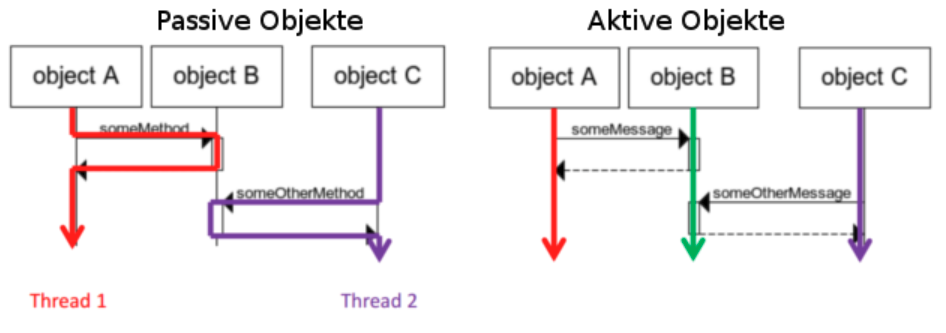
\includegraphics[width=0.9\linewidth]{img/passive_active_objects}
	\caption{Passive und Aktive Objekte}
	\label{fig:passiveactiveobjects}
\end{figure}

Ein Actor umfasst
\begin{itemize}
	\item Processing
	\item Storage
	\item Communication
\end{itemize}

Ein Actor kann
\begin{enumerate}
	\item Neue Actors erstellen
	\item Nachrichten an Actors (andere und sich selber) senden
	\item Entscheiden, wie die nächste Nachricht behandelt werden soll (Zustandsänderung)
\end{enumerate}

\newpage

\subsection{Communicating Sequential Processes (CSP )}

In CSP kommunizieren Prozesse indirekt über Channels, die Übermittlung von Nachrichten erfolgt zudem  unmittelbar und synchron.

Es ist ähnlich Actor Model, Unterschiede sind: 
\begin{itemize}
	\item Actor hat keine Channels
	\item Senden ist immer asynchron
	\item keine garantierte Reihenfolge des Empfangs
\end{itemize}

\begin{figure}[h!]
	\centering
	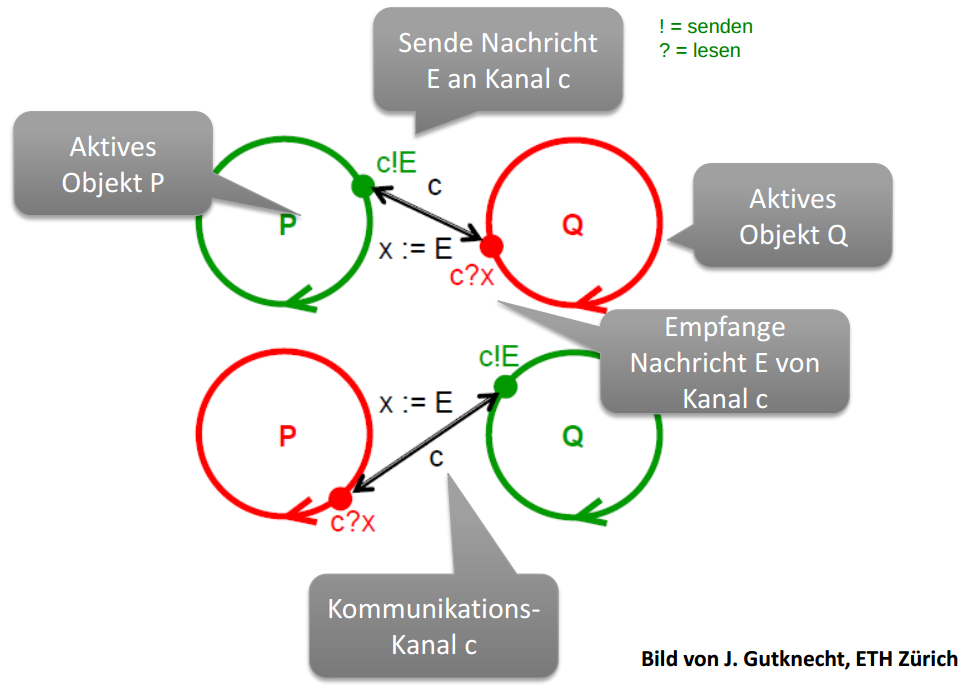
\includegraphics[width=0.7\linewidth]{img/csp_model}
	\caption{CSP Modell}
	\label{fig:cspmodel}
\end{figure}


\subsubsection{Vorteile von Actor und CSP}

\begin{itemize}
	\item Inhärente Nebenläufigkeit (alle Objekte (Actors) sind nebenläufig)
	\item Keine Race Conditions (kein shared memory)
	\item Gute Verteilbarkeit (Nachrichtenaustausch für Netz prädestiniert)
\end{itemize}

\subsubsection{Beispiel:}

\begin{lstlisting}
process A channel c {
	produce x;
	c!process(x)
}

process B channel c {
	c?process(x);
	consume x
}
\end{lstlisting}

\subsection{Actor implementierungen}

\begin{itemize}
	\item Erlang (1987): (z.B. WhatsApp nutzt Erlang im Backend)
	\item Akka \begin{itemize}
		\item Für JVM: Java, Scala, JRuby etc.
		\item Meta-Programmiermodell auf herkömmlicher Sprache
	\end{itemize}
	\item Java Communicating Sequential Processes (JCSP), veraltet!
	\item .NET \begin{itemize}
		\item Concurrency and Coordination Runtime CCR (low-level)
		\item Orleans (Microsoft Research, für Xbox eingesetzt)
		\item Akka.NET portierung für C\#
	\end{itemize}
\end{itemize}

\subsection{Akka}

Implementation in Scala (zusätzliches Java-API), gut für die Entwicklung nebenläufiger, verteilter, fehlertoleranter und event-basierter Systeme. Neben Erlang das verbreiteste Actor-Framework.

\subsubsection{Funktionalität}

\begin{itemize}
	\item Actor sind aktive Objekte, welche nebenläufig laufen
	\item Privater Zustand. Aufpassen, dass per Java Referenzen kein Share State entsteht! JVM forciert das nicht.
	\item Eine Mailbox pro Actor, ein Buffer pro Objekt mit asynchrones Senden. Geht an Methoden
	\item Intern sind Actors sequenziell.
\end{itemize}

\subsubsection{Anwendungsbereiche}

\begin{itemize}
	\item Alternative zu Threads
	\item Transaction-Processing
	\item Backend für Service (REST, SOAP, Websockets)
	\item Kommunikations-Hub (Router, Load Balancer)
\end{itemize}

\subsubsection{Codebeispiele}

\paragraph{Einfacher Actor} \hfill \\

\begin{lstlisting}[language=java]
public class NumberPrinter extends UntypedActor {
	public void onReceive(final Object message) {
		if (message instanceof Integer) {
			System.out.print(message);
		}
	}
}
\end{lstlisting}

\paragraph{Erzeugen und Senden} \hfill \\
Jeder Actor hat eine logische Adresse (Achtung: Hier ist nicht die Speicheradresse gemeint)

\begin{lstlisting}[language=java]
ActorSystem system = ActorSystem.create("System");

// Erzeugung per Reflection; ActorRef Immutable
ActorRef printer = system.actorOf(Props.create(NumberPrinter.class));

for (int i = 0; i < 100; i++) {
	printer.tell(i, ActorRef.noSender()); // Einfaches asynchrones Senden
}
system.shutdown(); // ''End-Signal'' an alle Actors
\end{lstlisting}

\subsubsection{Pattern: Producer-Consumer}

\begin{figure}[h]
	\centering
	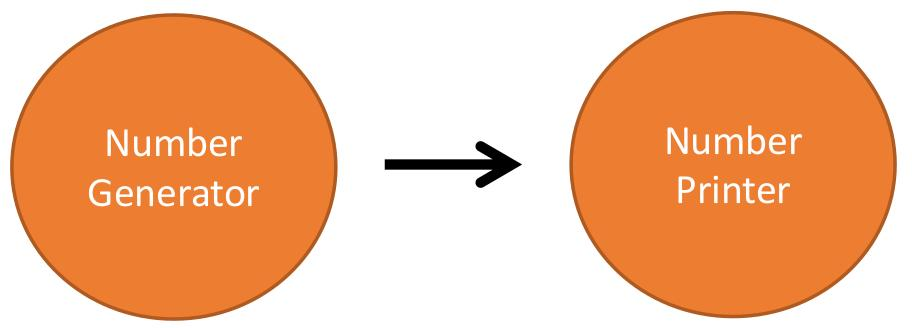
\includegraphics[width=0.5\linewidth]{img/akka_consumer_producer}
	\caption{Akka Consumer-Producer pattern}
	\label{fig:akkaconsumerproducer}
\end{figure}


\subsubsection{Pattern: Map-Reduce}

Aufteilung der Arbeit an mehrere Worker (''Map''), einsammeln und zusammenfügen der Resultate (''Reduce'')

\subsubsection{Netzwerk Verteilung}
Die Verteilung im Netzwerk ist relativ einfach, da der Code gleich bleibt und nur die ''application.conf'' angepasst werden muss.

\paragraph{Server} \hfill \\
\begin{lstlisting}[language=java]
ActorSystem system = ActorSystem.create("System");
ActorRef printer = system.actorOf(Props.create(...), "printer");
\end{lstlisting}

\begin{lstlisting}[language=java]
// application.conf
akka {
	actor {
		provider = "akka.remote.RemoteActorRefProvider"
	}
	remote {
		enabled-transports = ["akka.remote.netty.tcp"]
		netty.tcp {
			hostname = "server"
			port = 2552
		}
	}
}
\end{lstlisting}

\paragraph{Client} \hfill \\
\begin{lstlisting}[language=java]
ActorSystem system = ActorSystem.create("producer");
 // Selection ist leichgewichtiger als ActorRef, kann mehrere Actors umfassen
ActorSelection printer = system.actorSelection("akka.tcp://System@server:2552/user/printer");

printer.tell(123, ActorRef.noSender());
\end{lstlisting}

\paragraph{Hierarchie} \hfill \\

Die Hierarchie ist passend zum URL Adressierungsschema. Ein Parent ist automatisch ein Erzeuger. Es ist mit \lstinline|ActorSelection| möglich, einen Teilbaum zu selektieren und z.B. ein Broadcast zu senden. \lstinline|actorSelection("/usr/players");|

\subsubsection{Senden}

Es lassen sich Serializable / Immutable Objekte versenden.

\paragraph{Asynchron}
Der Absender muss bei jeder Message angegeben werden: \lstinline|tell(msg, sender)| A sendet an B, B leitet nur weiter. C antwortet direkt an A.

\begin{figure}[h]
	\centering
	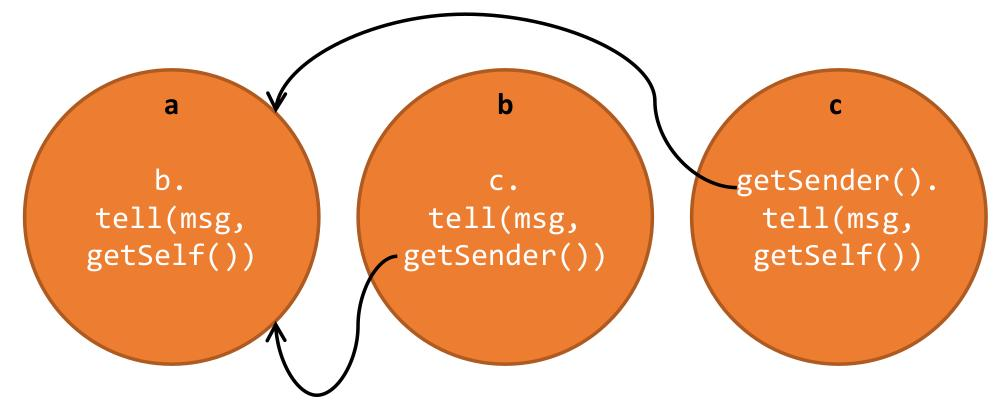
\includegraphics[width=0.7\linewidth]{img/akka_tell_asynchron}
	\caption{Akka tell() (Asynchron)}
	\label{fig:akkatellasynchron}
\end{figure}


\paragraph{Synchron} \hfill \\
Das Actor Modell ist standardmässig asynchron. Für synchrones Senden und Empfangen müssen Futures verwendet werden..
\begin{lstlisting}[language=java]
Future<Object> result = Patterns.ask(actorRef, msg, timeout);
\end{lstlisting}

Achtung: Durch synchrones arbeiten kann es bei falscher Anwendung zu Deadlocks kommen.

\subsubsection{Aktoren Supervision}

Actors können andere Actors überwachen und bei Exceptions den Supervisor benachrichtigen. Parents überwachen standardmässig ihre Kinder.

Supervisors können verschieden auf Fehler reagieren (sollte aber nur für externe Fehler genutzt werden, nicht Programmierfehler):
\begin{description}
	\item[Resume] Child macht weiter (behält interner Zustand)
	\item[Restart] Child wird neu gestartet (verliert Zustand)
	\item[Stop] Child wird nicht mehr ausgeführt
	\item[Escalate] Supervisor gibt auf und meldet selber seinem Supervisor einen Fehler
\end{description}

\paragraph{Root Guardian} \hfill \\
Der / in der URL ist der ''Root Guardian''. Er hat zusätzlich einen Unterknoten für \lstinline|/system| für Logging und Shutdowns).

\subsubsection{System shutdown}

\begin{lstlisting}[language=java]
getContext().stop(actorRef); // stopt nach bearbeitung der aktuellen message
getContext().stop(getSelf());
getContext().system().terminate();
actor.tell(PoisonPill.getInstance(), sender); // stoppen bei behandlung der Poison Pill
victim.tell(Kill.getInstance(), sender); // startet supervisor behandlung
\end{lstlisting}


\subsubsection{Schwächen}

\begin{itemize}
	\item Kein formales Kommunikationsprotokoll
	\item Akka: Keine Typsicherheit (welche Messages kann ein Aktor behandeln?)
	\item Akka: Diskrepanz JVM und Actor Model \begin{itemize}
		\item Shared Memory und Muability
		\item Brauche spezielle Referenzen zwischen Actors
		\item Leicht verletzbare Regeln $\rightarrow$ Laufzeitfehler.
	\end{itemize}
\end{itemize}

\subsubsection{Stärken}

\begin{itemize}
	\item Inhärente Nebenläufigkeit (Aktive Objekte)
	\item Keine Race Conditions (Aber Deadlocks und Starvations möglich)
	\item Leichte Verteilung (Kein Shared Memory), keine Data Races
	\item Challenge für Runtime \begin{itemize}
		\item Thread Pooling funktioniert nur bei ''Run-To-Completion'' Empfangsstil
		\item Braucht sonst neue  Art von Leichtgewichtsprozessen
	\end{itemize}
\end{itemize}


\section{GPU Parallelisiserung}

GPUs haben sehr viele Cores (meist tausende), und sind spezialisiert auf eine spezielle Art der Parallelisierung.


\subsection{GPU Architektur}

Bei CPUs nehmen die ALU nur einen kleinen Teil des Transistors ein, dafür sind sie sehr ausführlich; dafür steht viel Cache zur Verfügung.

Bei GPUs gibt es viele ALUs, welche aber weniger ausgefeilte Logik anbieten.

Streaming Multiprocoessors (eigentliche Cores), darin gibt es Streaming-Processors welche die eigentlichen ''Cores'' sind. (Dies sind aber nicht unabhängige Cores!)

\subsubsection{Streaming Multiprocessor}

Streaming Multiprocessor its prinzipiell SIMD (Single Instruction Multiple Data)
\begin{figure}[h]
	\centering
	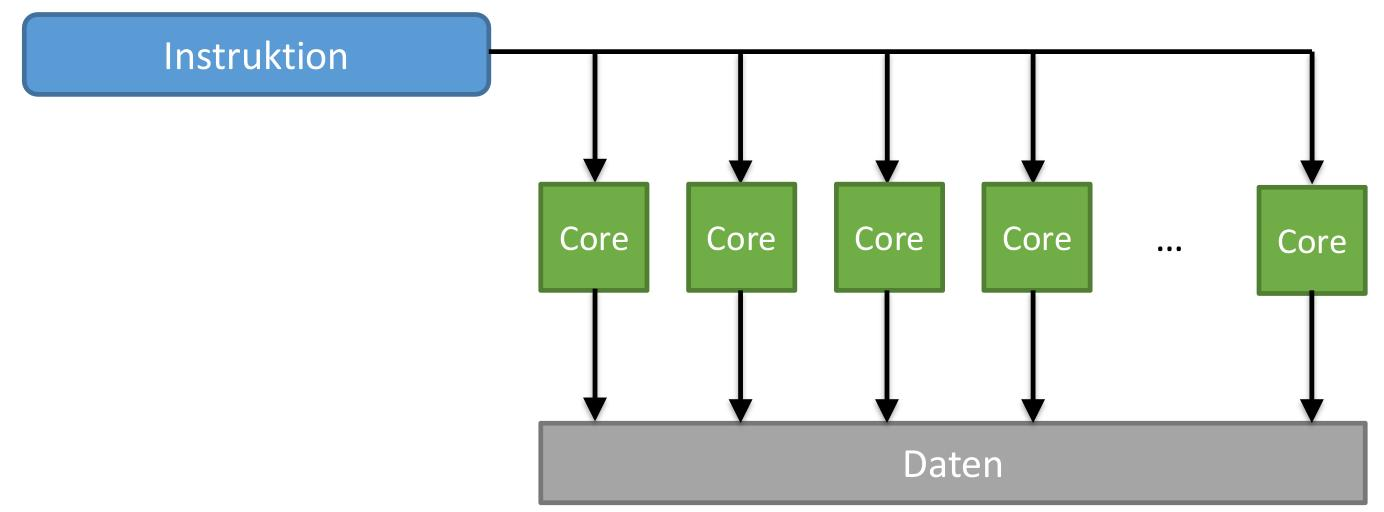
\includegraphics[width=0.7\linewidth]{img/simd_structure}
	\caption{SIMD Structure}
	\label{fig:simdstructure}
\end{figure}


SIMD Instruktionen führen zu parallelen Vektor-Operationen. Single instructure, multiple Data.

\begin{figure}[h]
	\centering
	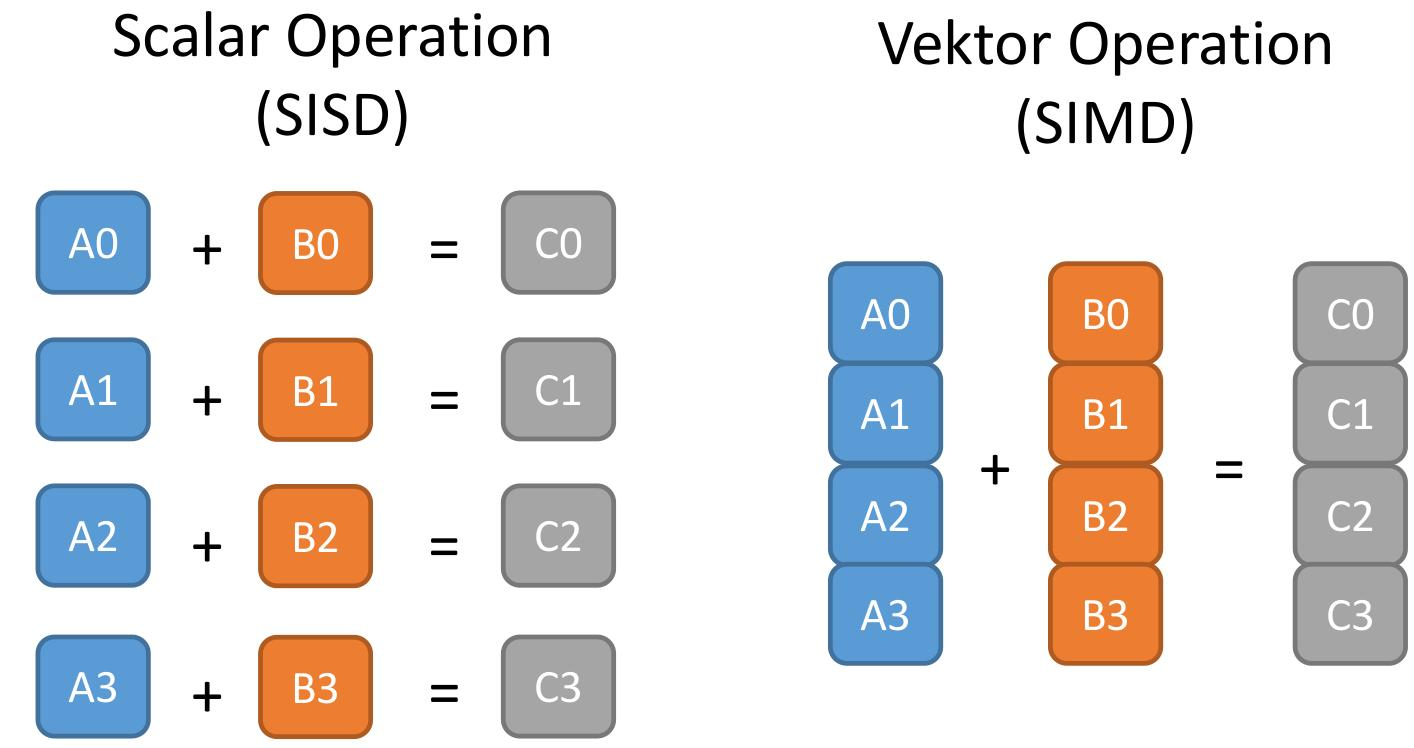
\includegraphics[width=0.7\linewidth]{img/simd_vektor.jpg}
	\caption{SIMD Vector Structure}
	\label{fig:simdvector}
\end{figure}

Streaming Multiprocessors untersützten auch eine virtuelle Parallelisierung, ähnlich den CPU-Threads.

\subsubsection{Nutzung}

Diese vielen parallelen Cores zu nutzen, ist meist eine Struktur mit Matrizen nötig.

\subsubsection{GPUs vs. CPUs}

\begin{figure}[h]
	\centering
	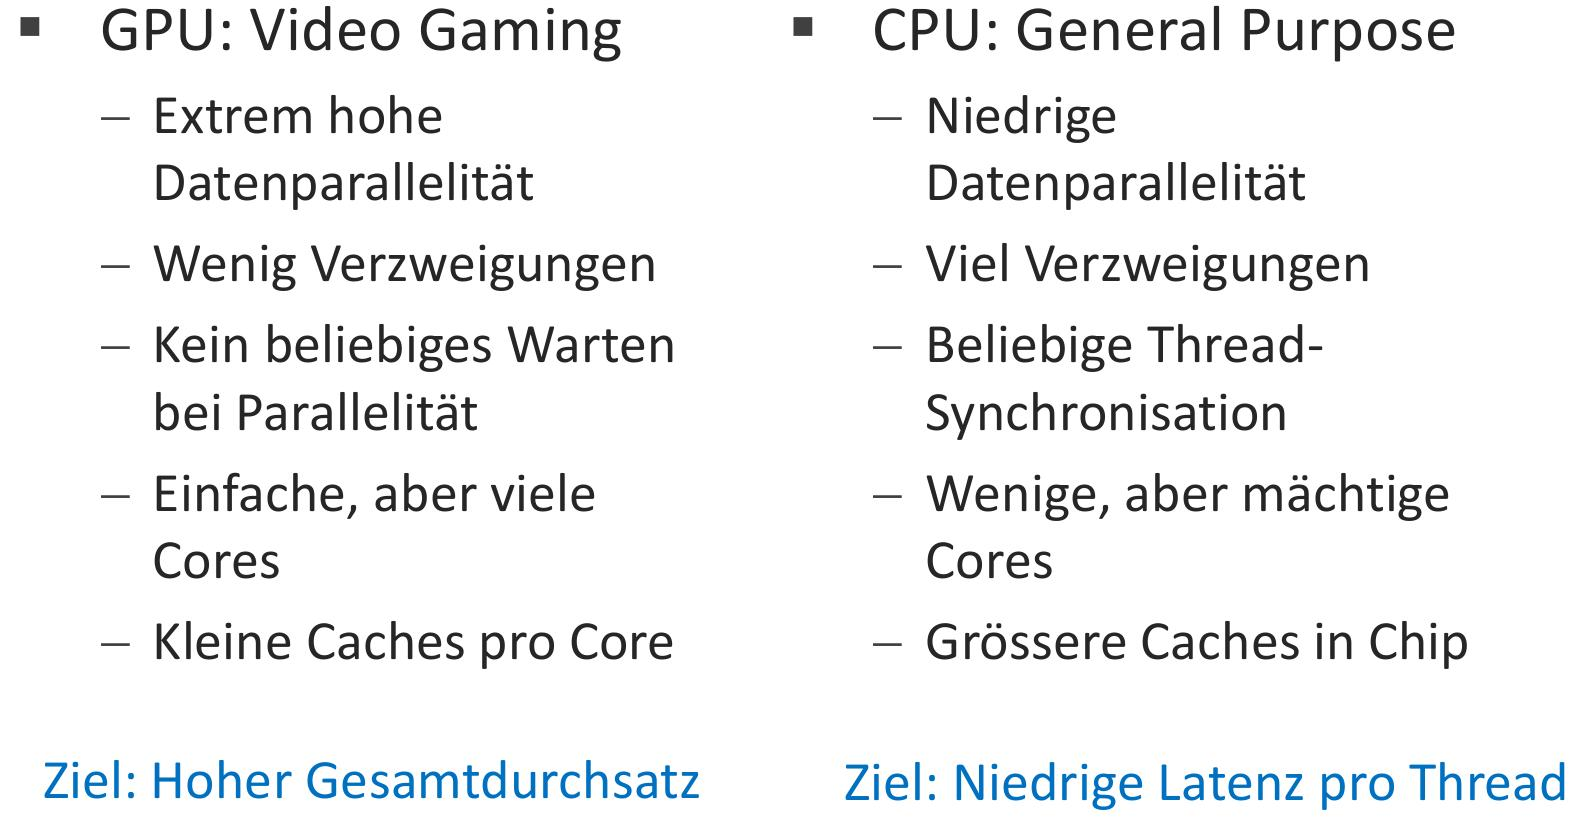
\includegraphics[width=0.7\linewidth]{img/gpu_vs_cpu.jpg}
	\caption{GPUs vs. CPUs}
	\label{fig:gpuvscpu}
\end{figure}

\subsubsection{NUMA Modell}

Der Grafikkarten-Speicher und Computer-Hauptspeicher sind im NUMA Modell getrennt. Daten müssen also immer übertragen werden.


\subsubsection{Programmierumgebungen}

Programmiermodelle:
\begin{itemize}
	\item CUDA: für NVIDIA Grafigkarten
	\item OpenCL: Unabhängiger Standard, ähnlich zu CUDA
	\item C++ AMP: Microsoft Technologie
	\item OpenACC: Offener Standard.
\end{itemize}

\subsection{CUDA}


Grundsätzlich wird jeder Thread = Kernel einzeln definiert. Threads sind in Blöcke gruppiert; ein Block läuft auf einem Streaming Multiprozessor. Ein Block kann sich untereinander synchronisieren, dies ist für höhere Ebenen nicht möglich, Blöcke müssen daher unabhängig sein. 

Es findet eine automatische Skalierung je nach Anzahl SM in der GPU.

Jeder Block hat eine ID, und Threads innerhalb von Blöcken

\begin{lstlisting}[language=C++]
// kernel definition: GPU
__global__
void VectorAddKernel(float *A, float *B, float *C) {
	int i = threadIdx.x;
	C[i] = A[i] + B[i];
}
int main() {
// kernel invocation
VectorAddKernel<<<1, N>>>(A, B, C);
}
\end{lstlisting}

\begin{figure}[h]
	\centering
	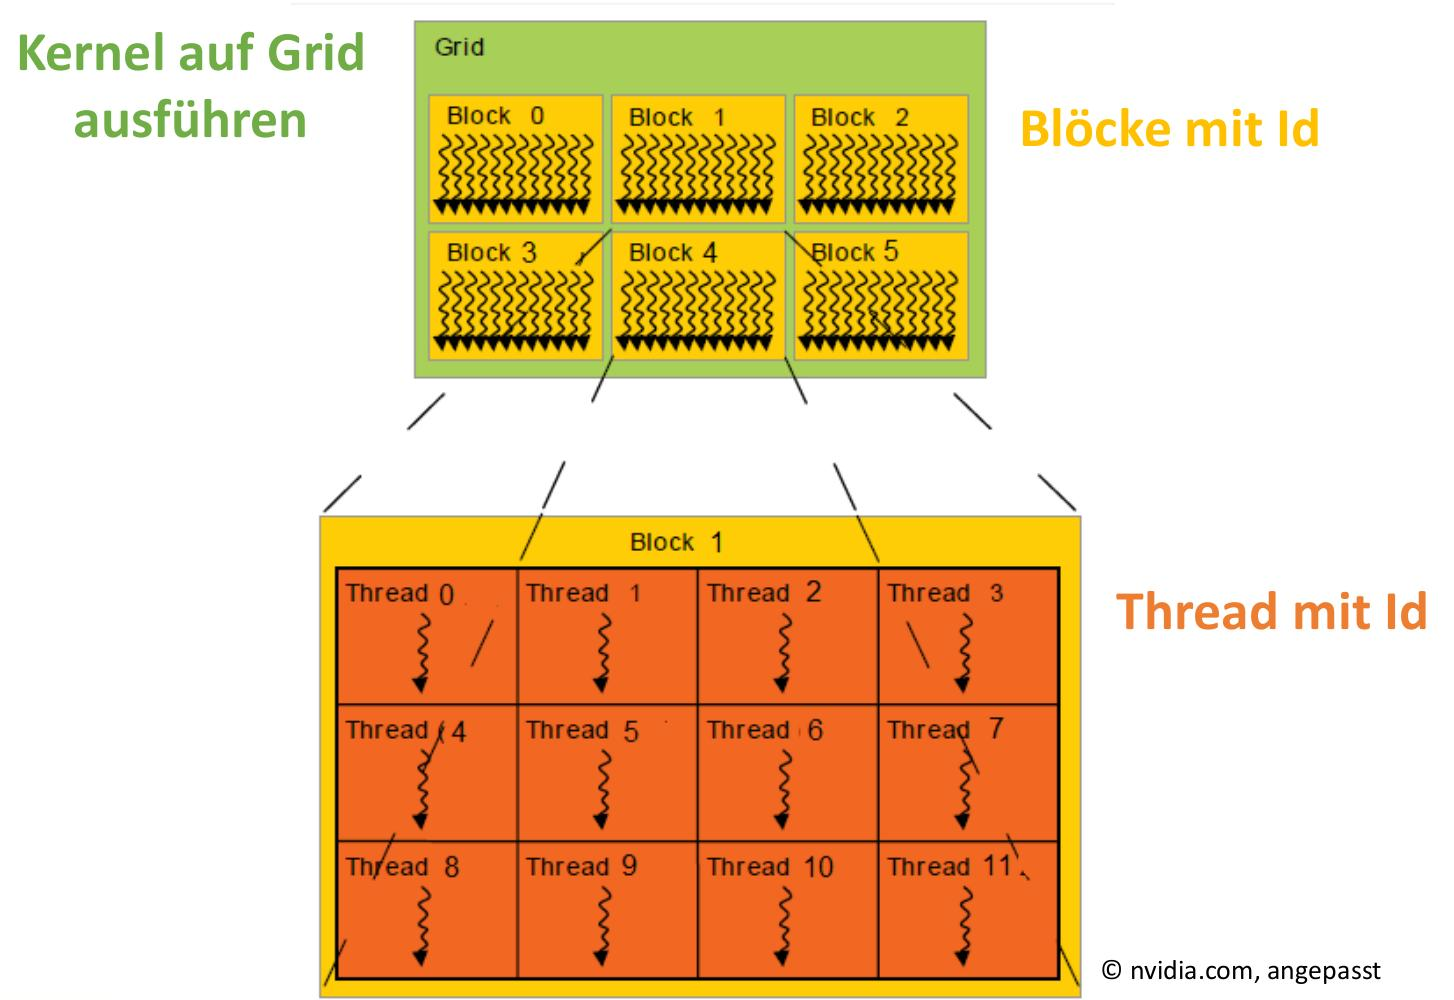
\includegraphics[width=0.7\linewidth]{img/gpu_thread_hierarchie.jpg}
	\caption{GPU Thread / Block Hierarchie}
	\label{fig:gputhradhierarchie}
\end{figure}

\begin{description}
	\item[threadIdx.x] Nummer des Threads innerhalb des Blocks
	\item[blockIdx.x] Nummer des Blocks
	\item[blockDim.x] Blockgrösse
	\item Weitere Dimensionen y, z nutzbar.
\end{description}

\lstinline|int i = threadIdx.x + blockDim.x * blockIdx.x|


\lstinline|VectorAddKernel<<<Bloecke, Threads pro Block>>>(A, B, C, 2048);|

\paragraph{Vernünftige Aufteilung in Blöcke:} \hfill \\

Die maximale ist abhängig von der GPU; sollte aber immer ein vielfaches von 32 sein, sonst ineffizient. Überflüssige Belegung sollte vermieden werden. Wenige grosse Blöcke sind aber auch effizienter als viele kleine.

Beim aufteilen sind auch die Anzahl Resident Blocks (die maximalen virtuellen Blocks) und die Anzahl Resident Threads (die maximale Anzahl Threads, welche gleichzeitig geladen werden können).

\begin{lstlisting}[language=C++]
__global__
void VectorAddKernel(float *A, float *B, float *C, int N) {
	int i = blockIdx.x * blockDim.x + threadIdx.x;
	if (i < N) { // Opt-Out bei ''Overflow'' (ist kostenmaessig billig)
		C[i] = A[i] + B[i];
	}
}

int blockSize = 512;
int gridSize = (N + blockSize - 1) / blockSize;
VectorAddKernel<<<gridSize, blockSize>>>(A, B, C, N);
\end{lstlisting}


\subsubsection{Memory management}

\paragraph{cudeMalloc} ist die Allokation von Memory auf der GPU

\begin{lstlisting}[language=C++]
size_t size = numElements * sizeof(float);
float *d_A;
cudaMalloc(&d_A, size);
\end{lstlisting}

\paragraph{cudeMemcpy} ist für das Kopieren von Memory von und nach dem GPU Memory

\begin{lstlisting}[language=C++]
cudaMemcpy(d_A, A, size, cudaMemcpyHostToDevice);
\end{lstlisting}


\paragraph{cudaFree} ist für das Freigeben von GPU Memory

\begin{lstlisting}[language=C++]
cudaFree(d_A);
\end{lstlisting}


\subsubsection{Fehlerbehandlung}

\begin{lstlisting}[language=C++]
cudaError error;
error = cudaMalloc(&d_A, size);
if (error != cudaSuccess) {
	fprintf(stderr, "Failed to allocate device vector A: %s\n",
		cudaGetErrorString(error));
	exit(EXIT_FAILURE);
}
\end{lstlisting}

oder ausgelagert in eine Hilfsmethode:

\begin{lstlisting}[language=C++]
void handleCudaError(cudaError error) {
	if (error != cudaSuccess) {
		fprintf(stderr, "CUDA: %s!\n",
			cudaGetErrorString(error));
		exit(EXIT_FAILURE);
	}
}
\end{lstlisting}

\subsubsection{Unified Memory (seit CUDA 6)}

\begin{lstlisting}[language=C++]
cudaMallocManaged(&A, size);
cudaMallocManaged(&B, size);
cudaMallocManaged(&C, size);

VectorAddKernel<<<..,..>>>(A, B, C, N);
cudaDeviceSynchronize();

cudaFree(d_A);
cudaFree(d_B);
cudaFree(d_C);
\end{lstlisting}


\subsection{CUDE II}

\subsubsection{3D-Thread Hierarchie}

\begin{lstlisting}[language=C++]
dim3 gridSize(3,2,1);
dims3 blockSize(4,3,1);
Call<<<gridSize, blockSize>>>();
\end{lstlisting}


\paragraph{C-Einschränkungen} \hfill \\

Keine mehrdimensionalen Arrays; \lstinline|float**| ist unfein, da Pointers.

In C\# oder Python ginge folgendes:
\begin{lstlisting}
float[,] matrix = new float[NofRows,NofCols];
matrix[row, col] = ...
\end{lstlisting}

In C manuelle Low-Level Linearisierung:
\begin{lstlisting}
float *matrix = (float *)malloc(NofRows * NofCols * sizeof(float));
matrix[row * NofCols + col] = ...;
\end{lstlisting}

\subsubsection{Matrix Multiplikation}
Bei fast allen Use-Cases von Grafikkarten Beschleunigung sind Matrizen im Spiel (z.B. Neuronale Netze, ML, Algorithmen etc.)

\paragraph{Sequenzielle Matrix Multiplikation}

\[
  C_{i,j} = \sum\limits^{K-1}_{0}{A_{i,k} \cdot B_{k,j}}
\]

\begin{figure}[h]
	\centering
	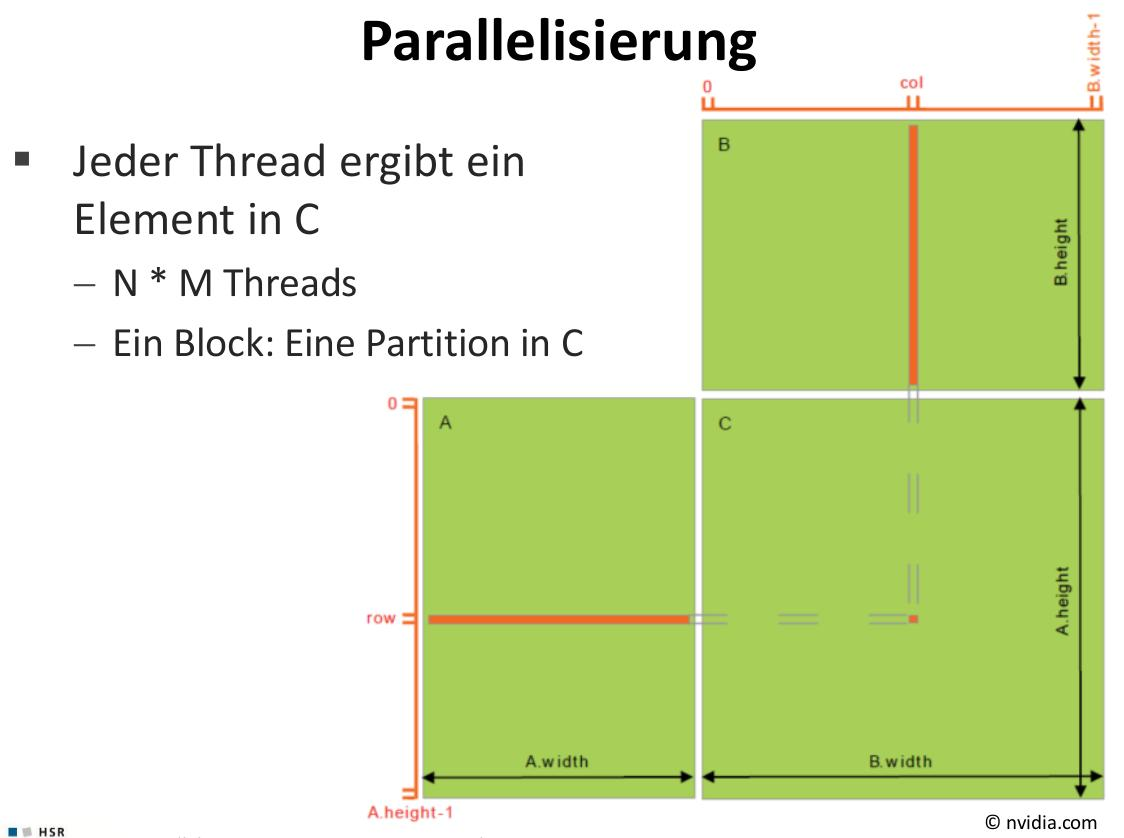
\includegraphics[width=0.7\linewidth]{img/gpu_matrix_multiplikation}
	\caption{GPU Matrix Multiplikation}
	\label{fig:gpumatrixmultiplikation}
\end{figure}


\begin{lstlisting}[language=C]
__global__
void matrixMultKernel(float *A, float *B, float *C) {
	int row = threadIdx.x + blockIdx.x * blockDim.x;
	int col = threadIdx.y + blockIdx.y * blockDim.y;
	if(row < C_ROWS && col < C_COLS) {
		float sum = 0;
		
		for(int k = 0; k < A_COLS; k++) {
			sum += A[rows * A_COLS + k] * B[k * B_COLS + col];
		}
			
		C[row * C_COLS + col] = sum;
	}
}

// Afuruf:

dim3 blockSize(32,32);
dim3 gridSize((C_ROWS + 31) / 32, (C_COLS + 31) / 32);
matrixMultKernel<<<gridSize,blockSize>>>(d_A, d_B, d_C);
\end{lstlisting}

Diese Lösung ist aber nicht sehr effizient; Memory Zugriffe sind eher teuer. Optimierungspotential: Die gleiche Spalte und Zeile wird ja an mehreren Orten mehrmals verwendet.

\subsubsection{Speicher und Memory}

\begin{figure}[h]
	\centering
	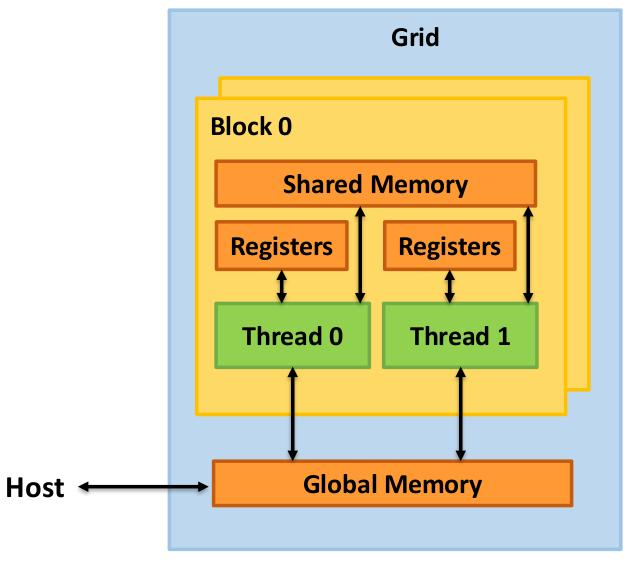
\includegraphics[width=0.7\linewidth]{img/gpu_memory_simplified}
	\caption{GPU Memory Layout (simplified)}
	\label{fig:gpumemorysimplified}
\end{figure}

\begin{figure}[h]
	\centering
	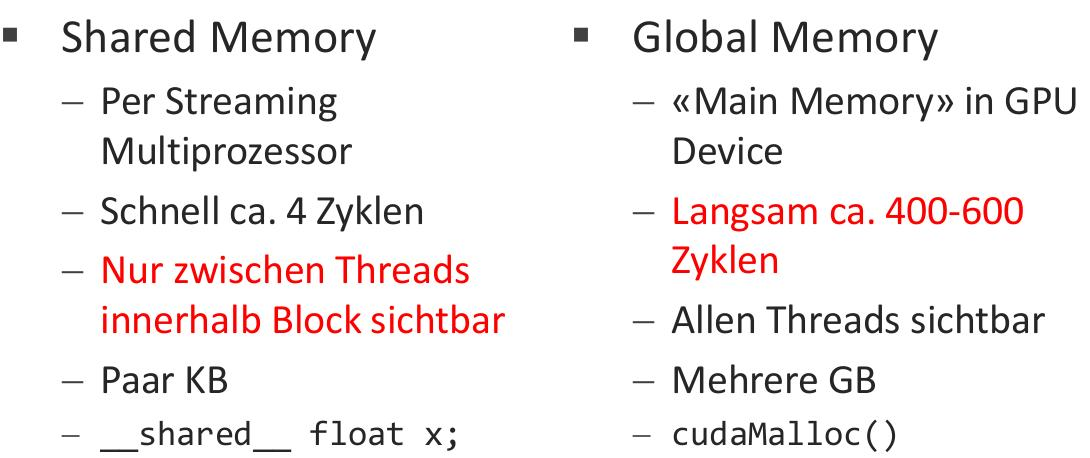
\includegraphics[width=0.7\linewidth]{img/gpu_memory_levels}
	\caption{GPU Memory Levels}
	\label{fig:gpumemorylevels}
\end{figure}


Es wäre Vernünftig, geteilte Spalten und Zeilen zu cachen. Dabei ist es von Vorteil, wenn der Bereich in C Quadratisch ist.


Erweiterung mit Cacheing:

\begin{lstlisting}[language=C]
__shared__ float Asub[TILE_SIZE][TILE_SIZE];
__shared__ float Bsub[TILE_SIZE][TILE_SIZE];

int tx = threadIdx.x, ty = threadIdx.y;
int col = blockIdx.x * TILE_SIZE + tx;
int row = blockIdx.y * TILE_SIZE + ty;

for (int tile = 0; tile < nofTiles; tile++) {
	Asub[ty][tx] = A[row * K + tile * TILE_SIZE + tx];
	Bsub[ty][tx] = B[(tile * TILE_SIZE + ty) * M + col];
	__syncthreads();
	for (int ksub = 0; ksub < TILE_SIZE; ksub++) {
		sum += Asub[ty][ksub] * Bsub[ksub][tx];
	}
	__syncthreads();
	// TODO: Hier gibt es noch keine Overflow / Fehlerbehandlung
}
C[row * M + col] = sum;
\end{lstlisting}


\subsubsection{Thread Synchronisation}


\lstinline|__syncthreads()| ist eine Barriere, damit alle Threads warten, bis der Cache gefüllt ist.

Wichtig: Syncthreads nie in if/else packen: Sind verschiedene Barrieren.

\subsubsection{Warps}

Ein Block wird intern in Warps zerlegt, zu je 32 Threads (darum immer Blöcke mit vielfachen von 32.)

Jeder Warp führt jeweils die gleiche Instruktion aus (nicht wirklich im ganzen Block...).

Ein Stream Multiprozessor kann alle Warps eines Blocks beherbergen.

Zur Latenzverringerung: Falls ein Warp auf Speicher wartet, führt der SM den nächsten Warp aus.

In einem Warp werden bei verschiedenen Pfaden von if/switch/while/do/for getrennt nacheinander ausgeführt:
\begin{lstlisting}[language=C]
if(threadIdx.x / 32 > 1) { /*...*/ } else { /*...*/ } 
\end{lstlisting}



\subsubsection{Memory Coalescing}

Speicher auslesen ist eher teuer. Durch Memory Burst kann das Abrufen aufeinander folgender Daten in einem Zugriff kombiniert werden. Hier kommt der 32 Threads block wieder ins Spiel. Der Zugriff muss immer auf 128 Byte aligned sein (bei Elementtyp >= 4Bytes)

Threads in Warp müssen Zugriffe auf alle Elemente einer Burst Section erledigen.

Dafür sollten Speicherzugriffe in die folgende Form umgeschrieben werden: \lstinline|data[(asdruck ohne threadIdx.x) + threadIdx.x]|



\section{Cluster}

Wir schauen hier in erster Linie wissenschaftliches Rechnen an.

\subsection{HPC (High-Performance Computing) Cluster Architektur}

Aufbau: Üblicherweise hat es einen Head Node (master) und Compute Nodes (slaves).

\begin{description}
	\item[Jobs] Zusammengehörende Tasks
	\item[Tasks] Ausführung eines Executables
\end{description}


Ziel: Ein Programm auf mehreren Nodes ausführen.

Zwei schwierigkeiten:
\begin{itemize}
	\item Kein Shared Memory (NUMA) zwischen Nodes
	\item Shared Memory (SMP) für Cores innerhalb Nodes
\end{itemize}


\subsection{MPI (Message Passing Interface)}

Basiert auf Actor Model/CSP-Prinzip, Industrie-üblich für massive Parallelisierung (z.B. Cluster, Multi-Core). Es gibt verschiedene Implementationen (MS HPC, MPICH)


\subsubsection{Beispiel in C\#.NET}

\begin{lstlisting}[language=C]
using MPI;
using System;
class Program {
	public static void Main(string[] args) {
		using (new MPI.Environment(ref args)) {
			int rank = Communicator.world.Rank;
			Console.WriteLine("MPI process {0} ", rank);
		}
	}
}
\end{lstlisting}

Ausführung mit: \lstinline|mpiexec -n 16 FirstMpiProgram.exe|

Nicht blockierendes senden:

\begin{lstlisting}[language=C]
var request = Communicator.world.ImmediateSend(text, right, 0);
Communicator.world.Receive(left, 0, out text);
request.Wait();
\end{lstlisting}

var request = Communicator.world.ImmediateSend(text, right, 0);
Communicator.world.

\subsubsection{Communikation}

MPI Elraubt es den Prozessen, untereinander zu kommunizieren.

Rank its die Nummer innerhalb der Gruppe und ist abfragbar mit \lstinline|Communicator.world.Rank|

Gesammtzahl der Prozesse: \lstinline|Communicator.world.Size|

\lstinline|Communiator.world|


\paragraph{Send}
\lstinline[language=C]|Communicator.world.Send(value, receiverRank, messageTag);|

\paragraph{Receive}
\lstinline[language=C]|Communicator.world.Receive(senderRank, messageTag, out value);|

\lstinline|messageTag|: Frei wählbare Nummer für Nachrichtenart (>= 0), üblicherweise immer gleich in einem Projekt. %TODO: Stimmt das so?


\paragraph{Barriere} \lstinline[language=C]|Communicator.world.Barrier()|


\paragraph{Reduktions-Funktionen}

\begin{description}
	\item[T Allreduce(T value, Op<T>)] \hfill \\
		Beliebige Aggregationsoperation (z.B. Lambda), jeder erhält das Gesamtresultat
	\item[T Reduce(T value, Op<T>, int rank)] \hfill \\
		Nur ein Prozess (Rank) sieht das Gesammtresultat, dadurch aber kein Broadcast $\rightarrow$ Effizienter
\end{description}


\section{Reactive Programming}

\subsection{Modell und Paradigma}

Beim Reactive Programming geht es darum, Datenflüsse zu Parallelisieren (Pipeline-Design)

\subsubsection{Klassischer Ansatz}

\begin{itemize}
	\item .NET LINQ (Parallelisierung auf .NET Task Parallel Library (TPL)
	\item Java 8 Stream API (Parallelisierung auf Fork Join Thread Pool)
\end{itemize}

\paragraph{Beispiel: Parallel LINQ (PLINQ)} \hfill \\
\begin{lstlisting}[language=SQL]
from entry in
	salesEurope.AsParallel()
	Union(salesAsia.AsParallel()).
	Union(salesAmerica.AsParallel())
group
	entry by entry.Article into category
	let sum = category.Sum(e => e.Volume)
where
	sum >= 1000
select
	new { category.Key, sum };
\end{lstlisting}


\paragraph{Lazy = Pull Mechanismus}

LINQ und Streams funktionieren nach dem Pull Mechanismus, d.h., die Daten werden ''herausgezogen'', die Pipeline schritte rückwärts ausgeführt. Die Input-Quelle ist dabei Passiv.

Bei Input-Pausen (User Input, Netzwerk etc.) sowie bei Streams unbekannter Länge funktioniert dieses Modell nicht richtig.

\subsubsection{Reactive = Push-Mechanismus}

Beim Reactive-Modell werden die Daten von einer verketteten Liste ausgeführt, welche auf Events basiert. Der Nachfolgeschritt abonniert die Events des Vorgängers (\lstinline|OnNext|)

\subsubsection{Rx.NET (Reactive Extensions)}

Rx.NET ist eigentlich Asynchrone Events + LINQ.

\begin{figure}
	\centering
	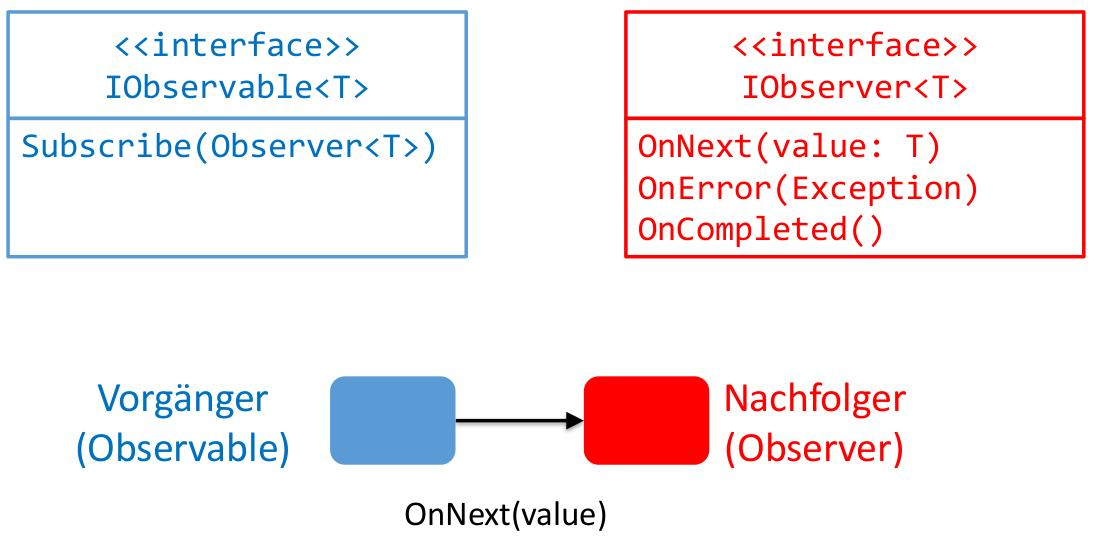
\includegraphics[width=0.7\linewidth]{img/rx_observer_pattern}
	\caption{Rx Observer Pattern}
	\label{fig:rxobserverpattern}
\end{figure}


\paragraph{Subject} = Observer + Observable. Oft auch ''Promise'' genannt.

Ein einfaches Beispiel:

\begin{lstlisting}[language=C]
var subject = new Subject<string>();
subject.Subscribe(
	x => Console.WriteLine($"First receiver {x}"),
	e => Console.WriteLine($"First receives error {e}"),
	() => Console.WriteLine("First sys bye bye!")
);

subject.OnNext("A");
subject.OnNext("B");


// Fehler ausloesen
subject.OnError(new Exception("FAIL"));

subject.OnNext("C");
subject.OnCompleted();

\end{lstlisting}


Bestehende Datenstrukturen können mit \lstinline|.ToObservable()| umgewandelt werden.

\begin{lstlisting}[language=C]
var combinedSales = salesEurope.ToObservable().Merge(salesAsia.ToObservable());
combinedSales.Subscribe(Console.WriteLine);
\end{lstlisting}

\paragraph{Parallelisierung} \hfill \\

\begin{lstlisting}[language=C]
observable.ObserveOn(TaskPoolScheduler.Default).Subscribe(...);
\end{lstlisting}

Mögliche Scheduler:
\begin{itemize}
	\item \lstinline|TaskPoolScheduler.Default| (Synchrone Ausführung)
	\item \lstinline|NewThreadScheduler.Default| (Aufrufe dieses Observable sind in neuem Thread)
	\item \lstinline|DispatcherScheduler.Current| (GUI-Thread)
\end{itemize}

\paragraph{Interaktion mit GUI} \hfill \\

combinedSales.ObserveOnDispatcher().Subscribe(
	entry =>
		textBlock.Text += entry.Article + " " + entry.Volume // Ausfuehrung auf GUI Thread
);

\subsection{Concurrency Aspekte}

Mögliche Fehler:

\begin{itemize}
	\item Race Conditions (Bei Seiteneffekten in Observer)
	\item Deadlocks (Bei Warteabhängigkeiten oder blockierende Aufurfe wie \lstinline|First()| oder \lstinline|Last()|
\end{itemize}


\subsection{Vorgefertigte Observables}

\begin{table}
	\lstset{linewidth=4.5cm}
	\begin{tabu}{X l}
		\lstinline|Observable.Return("Value")| & Liefert den Wert, dann Completed \\
		\lstinline|Observable.Empty()| & Liefert sofort Completed \\
		\lstinline|Observable.Never()| & Liefert nie etwas (auch nicht Completed) \\
		\lstinline|Observable.Throw(exception)| & Liefert sofort Error \\
		\lstinline|Observable.Range(-10, 20)| & Zahlen von -10 bis 10 \\
		\lstinline|Observable.Generate(0,v => v<100,v => v+2,v => v)| & Liefert 0, 2, 4, ..., 98 \\
		\lstinline|source.Take(10)| & Nächste 10 Werte von source, danach Completed \\
		\lstinline|Observable.Intervall(TimeSpan.FromMilliseconds(250))| & \\
		&  Liefert 0, 1, 2, .. im Zeit Intervall von 250 ms \\

		\lstinline|Observable.Timer(TimeSpan.FromDays(1))| & \\
		& Liefert «0» erst in einem Tag \\

		\lstinline|source.Delay(TimeSpan.FromSeconds(1))| & \\
		& Verzögert alle Werte von source einmal um 1 Sekunde
	\end{tabu}
\caption{Häufig benutzte Observable-Funktionen.}
\end{table}



\subsection{Nutzen und Limitationen}

\subsubsection{Hot \& Cold Observables}

Hot Observables haben eine Zeitkomponente, wohingegen Cold Observables passiv sind, wie Streams.


\subsection{Vor- und Nachteile}

\subsubsection{Vorteile}
\begin{itemize}
	\item Aktive Datenflüsse statt nur passive LINQ
	\item Skalierbare Parallelität durch Wahl der Scheduler
	\item Durchgängig asynchron
\end{itemize}


\subsubsection{Nachteile}
\begin{itemize}
	\item Zerstückelung komplexer Logiken in Handler
	\item Allfälliger Kontext muss durchgeschleust werden
	\item Komplizierte Aggregation (Observable statt Skalar)
\end{itemize}


\section{Transactional Memory}

Shared Mutable Memory kann u.a. leicht zu Deadlocks, Starvation und Race Conditions führen.

Software Transactional Memory (STM) ist eine Idee aus der Datenbankwelt, welche nicht zu Races, Deadlocks und Starvation führen soll. (Es gibt auch Hardware Transactional memory (HTM))


\subsection{Grundlagen}

Operationen sollen als atomare Sequenzen ausgeführt werden (ACI Transaktionen: Atomicity, Consistency, Isolation)

\begin{lstlisting}[language=java]
void deposit(int amount) {
	atomic {
		balance += amount;
	}
}
\end{lstlisting}

\subsubsection{Optimistic Concurrency: Typische Probleme}

Die Implementation ist meist Optimistic concurrency; damit gibt es Probleme z.B. bei Konsolenausgaben und Netzwerk/io, da dort ein Rollback nicht einfach ausgeführt werden kann.

Zudem besteht eine Starvation-Gefahr.


\subsubsection{Warten auf Bedingung in atomic}

\begin{lstlisting}[language=java]
void deposit(int amount) {
	atomic {
		if(balance < amount) {
			retry;
		}
		balance += amount;
	}
}
\end{lstlisting}



\subsubsection{Schnelle Rollbacks}

In einem \lstinline|atomic|-block sollte bei Fehlern sofort zurückgerollt werden, damit nicht allzu schwierige Konflikte entstehen.


\subsection{Java STM Framework}

\subsubsection{Beispiele}

\begin{lstlisting}[language=Java]
final Ref.View<Integer> balance = STM.newRef(0);
final Ref.View<LocalDate> lastUpdate = STM.newRef(LocalDate.now());
\end{lstlisting}

\paragraph{Transaktionen} \hfill \\
\begin{lstlisting}[language=Java]
import scala.concurrent.stm.japi.STM;
void deposit(int amount) {
	STM.atomic(() -> {
		balance.set(balance.get() + amount);
		lastUpdate.set(LocalDate.now());
	});
}
\end{lstlisting}

\paragraph{Retry} \hfill \\
\begin{lstlisting}[language=Java]
void withdraw(int amount) {
	STM.atomic(() -> {
		if (balance.get() < amount) {
			STM.retry();
		}
		balance.set(balance.get() - amount);
		lastUpdate.set(LocalDate.now());
	});
}
\end{lstlisting}


\paragraph{Nested Transactions} \hfill \\
\begin{lstlisting}[language=Java]
void transfer(BankAccount from, BankAccount to, int amount) {
	STM.atomic(() -> {
		from.withdraw(amount);
		to.deposit(amount);
	});
}
\end{lstlisting}


\paragraph{Exceptions} Rollback und abbrechen, kein Retry. \hfill \\
\begin{lstlisting}[language=Java]
void deposit(int amount) {
	STM.atomic(() -> {
		if (balance.get() >= Limit) {
			throw new RuntimeException("Balance limit");
		}
		balance.set(balance.get() - amount);
		lastUpdate.set(LocalDate.now());
	}
}
\end{lstlisting}

\subsubsection{Einschränkungen}

z.B. ein \lstinline|Ref.View<Map<K, V>>| ist nicht Transaktionssicher. Es muss z.B. ein \lstinline|STM.newMap();| verwendet werden.

Seiteneffekte und externe Ressourcen sind aus atomic-Blöcken nicht möglich

\subsection{Probleme}

\subsubsection{Write Skew Problem}

Meist werden bei Transaktionellen Systemen Entscheidungen aufgrund von ''snapshots'' getroffen. D.h. ein \lstinline|if| arbeitet mit den Informationen, welche zum Anfang vorhanden waren.

\paragraph{Beispiel:} \hfill \\
\begin{lstlisting}[language=java]
atomic {
	if (a.onDuty) {
		b.onDuty = false;
	}
}
// concurrent:
atomic {
	if (b.onDuty) {
		a.onDuty = false;
	}
}
\end{lstlisting}


\subsubsection{Starvation}

Starvation ist fast immer möglich. (Es gibt keine elegante Lösung für dieses Problem.)


\appendix

% Code Listings
\lstlistoflistings

% List of figures
\listoffigures

% List of tables
\listoftables

% Bibliography
\bibliographystyle{plain} 
\bibliography{literatur}

\end{document}